\documentclass[sigconf]{acmart}

\usepackage{booktabs} % For formal tables
\usepackage{listings}
\usepackage{times}
\usepackage{makecell}


\newcommand{\eat}[1]{}
\settopmatter{printacmref=false}
\eat{
% DOI
\acmDOI{10.475/123_4}

% ISBN
\acmISBN{123-4567-24-567/08/06}
}

%Conference
\acmConference[Under Review]{}
\acmYear{2017}
%\copyrightyear{2017}

\eat{
\acmArticle{4}
\acmPrice{15.00}

% These commands are optional
%\acmBooktitle{Transactions of the ACM Woodstock conference}
\editor{Jennifer B. Sartor}
\editor{Theo D'Hondt}
\editor{Wolfgang De Meuter}
}

\begin{document}
\title{PlinyCompute: A Platform for High-Performance, Distributed,
  Data-Intesive Tool Development}
\eat{
\titlenote{Produces the permission block, and
  copyright information}
\subtitle{Extended Abstract}
\subtitlenote{The full version of the author's guide is available as
  \texttt{acmart.pdf} document}


\author{Ben Trovato}
\authornote{Dr.~Trovato insisted his name be first.}
\orcid{1234-5678-9012}
\affiliation{%
  \institution{Institute for Clarity in Documentation}
  \streetaddress{P.O. Box 1212}
  \city{Dublin} 
  \state{Ohio} 
  \postcode{43017-6221}
}
\email{trovato@corporation.com}

\author{G.K.M. Tobin}
\authornote{The secretary disavows any knowledge of this author's actions.}
\affiliation{%
  \institution{Institute for Clarity in Documentation}
  \streetaddress{P.O. Box 1212}
  \city{Dublin} 
  \state{Ohio} 
  \postcode{43017-6221}
}
\email{webmaster@marysville-ohio.com}

\author{Lars Th{\o}rv{\"a}ld}
\authornote{This author is the
  one who did all the really hard work.}
\affiliation{%
  \institution{The Th{\o}rv{\"a}ld Group}
  \streetaddress{1 Th{\o}rv{\"a}ld Circle}
  \city{Hekla} 
  \country{Iceland}}
\email{larst@affiliation.org}

\author{Valerie B\'eranger}
\affiliation{%
  \institution{Inria Paris-Rocquencourt}
  \city{Rocquencourt}
  \country{France}
}
\author{Aparna Patel} 
\affiliation{%
 \institution{Rajiv Gandhi University}
 \streetaddress{Rono-Hills}
 \city{Doimukh} 
 \state{Arunachal Pradesh}
 \country{India}}
\author{Huifen Chan}
\affiliation{%
  \institution{Tsinghua University}
  \streetaddress{30 Shuangqing Rd}
  \city{Haidian Qu} 
  \state{Beijing Shi}
  \country{China}
}

\author{Charles Palmer}
\affiliation{%
  \institution{Palmer Research Laboratories}
  \streetaddress{8600 Datapoint Drive}
  \city{San Antonio}
  \state{Texas} 
  \postcode{78229}}
\email{cpalmer@prl.com}

\author{John Smith}
\affiliation{\institution{The Th{\o}rv{\"a}ld Group}}
\email{jsmith@affiliation.org}

\author{Julius P.~Kumquat}
\affiliation{\institution{The Kumquat Consortium}}
\email{jpkumquat@consortium.net}

% The default list of authors is too long for headers.
\renewcommand{\shortauthors}{B. Trovato et al.}
}

\begin{abstract}
This paper describes \emph{PlinyCompute}, a system for development of
high-performance, data-intensive, distributed computing tools and libraries.
Currently, there is a big gap in performance and functionality between 
high-performance computing platforms such as OpenMP and MPI, which provide little direct support for
managing very large datasets, and dataflow platforms such as Spark and Flink.  Spark and Flink
are built to process large datasets but are themselves constructed on top of the
Java Virtual Machine (JVM), and hence must
at least partially cede concerns such as 
memory management (including layout and de/allocation) and virtual method/function dispatch to the JVM. Since memory management 
and the frequency of virtual function calls are
among the most important factors determining system performance,
this can have a very high cost.

PlinyCompute (or PC for short) is designed to occupy the space between these two 
existing classes of systems, providing high-performance, distributed, data-oriented computing with an expressive,
object oriented programming interface.
PC differs from other systems in that \emph{in the large}, it presents the programmer with a very high-level,
declarative interface, relying on automatic, relational-database style optimization to figure out how to stage
distributed computations.  However, \emph{in the small}, PlinyCompute presents the capable systems programmer with a
persistent object data model and API (the ``PC object model'') and associated memory management system
that has been designed from the ground-up for
high performance distributed, data-oriented computing.
PC's execution engine is not merely implemented on top of
PC object model.  Rather, the two have been co-designed to offer the best possible efficiency.
This hybrid approach---declarative in the large, trusting the programmer's ability
to utilize PC object model efficiently
in the small---results in a system that is ideal for the development of reusable, data-oriented tools and libraries.
Through extensive benchmarking, we show that implementing non-trivial, library-style computations 
on top of PC can result in a speedup of 2$\times$ to
more than 
50$\times$ or more compared to an identical implementation on Spark.
\end{abstract}


%
% The code below should be generated by the tool at
% http://dl.acm.org/ccs.cfm
% Please copy and paste the code instead of the example below. 
%
\eat{
\begin{CCSXML}
<ccs2012>
 <concept>
  <concept_id>10010520.10010553.10010562</concept_id>
  <concept_desc>Computer systems organization~Embedded systems</concept_desc>
  <concept_significance>500</concept_significance>
 </concept>
 <concept>
  <concept_id>10010520.10010575.10010755</concept_id>
  <concept_desc>Computer systems organization~Redundancy</concept_desc>
  <concept_significance>300</concept_significance>
 </concept>
 <concept>
  <concept_id>10010520.10010553.10010554</concept_id>
  <concept_desc>Computer systems organization~Robotics</concept_desc>
  <concept_significance>100</concept_significance>
 </concept>
 <concept>
  <concept_id>10003033.10003083.10003095</concept_id>
  <concept_desc>Networks~Network reliability</concept_desc>
  <concept_significance>100</concept_significance>
 </concept>
</ccs2012>  
\end{CCSXML}

\ccsdesc[500]{Computer systems organization~Embedded systems}
\ccsdesc[300]{Computer systems organization~Redundancy}
\ccsdesc{Computer systems organization~Robotics}
\ccsdesc[100]{Networks~Network reliability}


\keywords{ACM proceedings, \LaTeX, text tagging}

}
\maketitle
\definecolor{dkgreen}{rgb}{0,0.6,0}
\definecolor{gray}{rgb}{0.5,0.5,0.5}
\definecolor{mauve}{rgb}{0.58,0,0.82}

\lstnewenvironment{code}
  {\lstset{
        aboveskip=10pt,
        belowskip=10pt,
        %aboveskip=9pt,
        %belowskip=9pt,
        xleftmargin=15pt,        
        escapechar=!,
        mathescape=true,
        language=C++,
        %basicstyle=\linespread{0.94}\ttfamily\small,
        basicstyle=\linespread{0.94}\ttfamily\footnotesize,
	    morekeywords={createSet, sendData, makeLambdaFromMember,
		execute, setInput, setOutput, makeLambda, makeLambdaFromMethod, 
		Handle, Vector, Map, pair, makeObjectAllocatorBlock, push_back, Object, makeObject},
        keywordstyle=\color{blue}\ttfamily,
        stringstyle=\color{mauve}\ttfamily,
        commentstyle=\color{dkgreen}\ttfamily,			
        showstringspaces=true}
        \vspace{0pt}%
        \noindent\minipage{0.47\textwidth}}
  {\endminipage\vspace{0pt}}



\lstnewenvironment{codesmall}
  {\lstset{
        aboveskip=10pt,
        belowskip=10pt,
        %aboveskip=9pt,
        %belowskip=9pt,
        xleftmargin=15pt,        
        escapechar=!,
        mathescape=true,
        language=C++,
        basicstyle=\linespread{0.94}\ttfamily\footnotesize,
	    morekeywords={createSet, sendData, makeLambdaFromMember,
		hash, join, APPLY, FILTER, execute, setInput, setOutput, makeLambda, makeLambdaFromMethod, 
		Handle, Vector, Map, pair, makeObjectAllocatorBlock, push_back, Object, makeObject},
        keywordstyle=\color{blue}\ttfamily,
        stringstyle=\color{mauve}\ttfamily,
        commentstyle=\color{dkgreen}\ttfamily,            			
        showstringspaces=true}
        \vspace{0pt}%
        \noindent\minipage{0.47\textwidth}}
  {\endminipage\vspace{0pt}}



% http://www.vldb.org/pvldb/vol9/p1707-pirk.pdf
% https://cs.stanford.edu/~matei/papers/2017/cidr_weld.pdf
% http://www.vldb.org/pvldb/vol7/p853-klonatos.pdf

\section{Introduction}
Big Data systems such as Spark \cite{zaharia2010spark} and Flink \cite{alexandrov2014stratosphere, carbone2015apache}
have effectively solved what we call the ``data munging'' problem.  That is, 
these systems do an excellent job supporting the rapid
and robust development of problem-specific,
distributed/parallel codes that transform a raw dataset into structured 
or semi-structured form, and then
extract actionable information from the transformed data.
But while existing Big Data systems offer
excellent support for data munging,
there is a class of application for which 
existing systems are 
used, but arguably are far less suitable:
as a platform 
for the development of high-performance codes, especially reusable
Big Data tools and libraries, by a capable
system programmer.

The desire to build new tools
on top of existing Big Data systems is understandable.  
The  developer of a distributed data processing tool must worry about data persistence, movement of
data to/from secondary storage, data
and task distribution, resource allocation, load balancing, fault tolerance, and many other factors.
While classical high-performance computing (HPC)
tools such as MPI \cite{gropp1996high} do not provide support for all of these concerns,
existing Big Data systems 
address them quite well.
As a result, many tools and libraries have been built on top of existing systems.  For example,
Spark supports
machine learning (ML) libraries Mahout \cite{mahout}, Dl4j \cite{dj4j}, 
and Spark \texttt{mllib} \cite{meng2016mllib}, linear algebra packages such as SystemML \cite{tian2012scalable, boehm2016systemml, ghoting2011systemml, boehm2014hybrid} and Samsara \cite{samsara}, and graph analytics with
GraphX \cite{gonzalez2014graphx} and GraphFrames
\cite{dave2016graphframes}.  Examples abound.

\vspace{5 pt}
\noindent
\textbf{PlinyCompute: A platform for high-performance, Big Data computing.}
However, we assert that if one were to develop a system purely for developing high-performance
Big Data codes
by a capable systems programmer,
it would not look like existing systems such as Spark, Flink,
DryadLinq~\cite{yu2008dryadlinq} and so on, 
which have largely 
been built using high-level programming languages and managed runtimes
such as the JVM and the .NET Common Language
Runtime (CLR).  Managed runtimes abstract away
most details regarding memory management
from the system designer, including memory allocation, deallocation,
reuse, and movement, as well as virtual function dispatch, 
object layout.
Since managing and utilizing memory is 
one of the most important factors determining big data system performance, reliance
on a managed environment can mean an order-of-magnitude increase in CPU cost for some computations~\cite{blackburn2006dacapo}.  
This cost may be acceptable if the person using the system
is a programmer uncomfortable with the basics of memory management who is
building an application to complete a specific data munging task.  
But it is unacceptable for high-performance tool or library
development by an expert. There have been notable efforts to engineer around the limitations of a managed environment and still provide
high performance---Spark's Dataset and
Dataframe abstractions come to mind---but such efforts are necessarily limited compared to
designing a Big Data system from the ground up around special-purpose
memory and object management system.

This paper is concerned with the design and implementation of
\emph{PlinyCompute}, a system for development of
high-performance, data-intensive, distributed computing codes, especially tools and libraries.
PlinyCompute, or PC for short, is designed to fill the gap between
HPC softwares such as OpenMP \cite{dagum1998openmp} and MPI \cite{gropp1996high}, which provide little direct support for
managing very large datasets, and dataflow platforms such as Spark and Flink, which 
may give up significant performance through their reliance on a managed runtime to handle
memory management (including layout and de/allocation) and key computational considerations
such as virtual function dispatch. 

\vspace{5 pt}
\noindent
\textbf{Core design principle: Declarative in the large, high-performance in the small.}
PC is unique in that \emph{in the large}, 
it presents the programmer with a very high-level,
declarative interface, relying on automatic, 
relational-database style optimization \cite{chaudhuri1998overview} to figure out how to stage
distributed computations.  
PC's declarative interface is higher-level than other Big Data systems
such as Spark and Flink, in that decisions such as choice of join ordering and which
join algorithms to run are
totally under control of the system. 
This is particularly important for tool and library development because the same tool should run well regardless of the data
it is applied to---the classical idea of \emph{data independence} in database system design \cite{stonebraker1990third}.
A relatively naive library user cannot be expected to tune a library implementation of an algorithm to run
well on his or her particular dataset, and yet with existing systems, this sort of tuning
is absolutely necessary.  For example, we find
that a high quality LDA implementation\footnote{LDA \cite{blei2003latent} is a popular text mining algorithm.}
on top of Spark is around $25\times$ slower than the algorithmically equivalent LDA
implementation on top of PC.  Through careful, dataset-specific tuning (including choosing specific join algorithms and
forcing pipelining of certain results) it is possible to get that gap down to $2.5\times$.  But this requires modification of the
code itself, which is beyond the vast majority of end-users.

In contrast, \emph{in the small}, PlinyCompute presents a capable programmer with a
persistent object data model and API (the ``PC object model'') and associated memory management system
designed from the ground-up for
high performance.
All data processed by PC are managed by
the PC object
model, which is exclusively responsible for PC data layout and within-page memory management.  
The PC object model is tightly coupled with
PC's execution engine, and has been specifically designed for
efficient distributed computing.  
All dynamic PC \texttt{Object} allocation is \emph{in-place}, directly on a page, obviating
the need for PC \texttt{Object} serialization and deserialization before data are transferred to/from storage or over a network.
Further, PC gives a programmer fine-grained control of the systems
memory management and PC \texttt{Object} re-use policies.

This hybrid approach---declarative and yet trusting the programmer
to utilize PC's object model effectively
in the small---results in a system that is ideal for the 
development of data-oriented tools and libraries.


The system consists of following components: 

\begin{itemize}
\item The \textbf{PC object model}, which is a toolkit for building high-performance, persistent data structures that can be 
processed and manipulated by PC.  

\item The \textbf{PC API and TCAP compiler}.  In the large, PC codes
  are declarative and look a lot like classical relational calculus
  \cite{codd1971data}.  For example, to specify a join over five sets
  of objects, a PC programmer does not build a join directed acyclic
  graph (DAG) over the five inputs, as in a standard
dataflow platform.  Rather, a programmer 
supplies two \emph{lambda term construction functions}: one that constructs a lambda term describing the selection
predicate over those five input sets, 
and a second that constructs a lambda term describing the relational projection over those five sets
using the same API.  These lambda terms are constructed using PC's built-in lambda abstraction families as well as higher-order composition functions.
 PC's TCAP compiler 
accepts such a specification, and compiles it into a functional, domain specific language called \emph{TCAP} that implements
the join.  Logically, TCAP operates over
sets of columns of PC \texttt{Object}s. 

\item The \textbf{execution engine}, which is a distributed query processing
  system for big data analytics. It consists of an optimizer for TCAP
  programs and a high-performance, distributed, vectorized TCAP
  processing engine.  
The TCAP processing engine has been designed to work closely with the PC object model to
minimize memory-related costs during computation.

\item \textbf{Various distributed services}, which include a catalog
  manager serving system meta-data, and a distributed storage manager.



\end{itemize}

\vspace{5 pt}
\noindent
\textbf{Our contributions.}
Taken together, these components allow a competent system programmer to write exceedingly high-performance distributed codes.
In this paper, we describe the design and implementation of PlinyCompute.  Currently, PC exists as a prototype system, consisting of around
150,000 lines of C++ code, with a much smaller amount of Prolog code. We experimentally show the performance benefits of the PC object model, 
demonstrating how even simple data transformations are much faster using the PC object model compared to similar computations within the 
Apache ecosystem.
In keeping with PC being targeted at high-performance
library and tool development,
we benchmark several library-style softwares written on top of PC.  We begin with a small domain specific language
for distributed linear algebra that we implemented on top of PC, called \texttt{LilLinAlg}.  \texttt{LilLinAlg} was implemented in about six weeks by a developer
who had no knowledge of PC at the outset, with the goal of demonstrating PC's suitability as a tool-development platform.  
We show that \texttt{LilLinAlg} has better performance than other systems that have long been under development
within the Apache ecosystem.   
We also benchmark the efficiency of manipulating complex objects, and
several standard machine learning codes written on top of PC.  

\vspace{5 pt}
\noindent
\textbf{Roadmap.} We first present an overview of PC runtime and the key components
: the PC object model, the lambda calculus that
forms the basis of PC API, 
and TCAP and PC's execution engine. Then we discuss PC object model
and TCAP optimization
in more detail in Section~\ref{sec:ObjectModel}  and
Section~\ref{sec:optimizer} respectively. In
Section~\ref{sec:exp}, we present a thorough 
evaluation and demonstrates that PlinyCompute outperforms alternatives
in building non-trivial, library-style computations  and manipulating
complex objects. Finally, we discuss related works in
Section~\ref{sec:survey} and summarize the paper in Section~\ref{sec:conc}.

\section{PlinyCompute Overview}

The PC software consists of 
(1) the PC object model, (2) the PC API and TCAP compiler (TCAP is a domain-specific language executed by PC),
(3) the execution engine, and (4) various distributed services.  In the next few sections of the paper, 
we discuss the first three software components in detail.

When PC runs on a distributed cluster it has a \emph{master node} and one or more \emph{worker nodes}.
Running on the master node are the managers for the various distributed services provided by PC, primarily 
the \emph{catalog manager} and the \emph{distributed storage manager}.  Also running on the master
node is the software responsible for powering the distributed execution engine: the \emph{TCAP optimizer} and
the \emph{distributed query scheduler}.  
When a user of PC requests to execute a graph of computations, the
computations are compiled into a TCAP program on the user's process, then optimized
by the master node's TCAP optimizer and executed by the distributed query scheduler.

Each worker node runs two processes: the \emph{worker front-end process} and the \emph{worker backend process}.
Dual processes are used because the backend process
executes potentially unsafe native user code.
If
user code happens to crash the worker backend process, the worker 
front-end process can re-fork the worker
backend process.  
The worker front-end process interfaces with the master node, providing a local catalog manager and a local storage server (including
a local buffer pool)
and crucially, it acts as a proxy, forwarding requests to perform various computations to the worker backend process, where
computations are actually run.

\section{Object Model Overview}

There is growing evidence that the CPU costs associated with manipulating data, especially data (de-)serialization and memory 
(de-)allocation,  
dominate the time needed to complete typical big data processing tasks
\cite{ousterhout2015making, shi2015clash, SikdarSoCC2017}.
To avoid these potential pitfalls while at the same time giving the user a high degree of flexibility,
PC requires programmers to store and manipulate data using the \emph{PC object model}.
The PC object model is an API for storing and manipulating objects, and has been co-designed with PC's memory management system and execution engine to provide
maximum performance.  

In PC's C++ binding, individual PC \texttt{Object}s correspond to C++ objects, and so the C++ compiler specifies the memory layout.
However, where PC \texttt{Object}s are stored in RAM and on disk, and how they are allocated and deallocated, when and where they are moved, is
tightly controlled by PC itself.

The PC object model provides a fully object-oriented interface, and yet manages to avoid many of the costs associated with complex object manipulation
by following the \emph{page-as-a-heap} principle.  
All PC \texttt{Object}s are allocated and manipulated in-place, on a system-
(or user-) allocated page.  There is
no distinction between the in-memory representation of data and the on-disk (or in-network) representation of
data. Thus there is no (de-)serialization cost to move data to/from disk and network, and memory management costs are very low. Depending upon choices made by the
programmer, ``deallocating'' a page of objects
means simply unpinning the page and allowing it to be returned to the buffer
pool, where it will be recycled and written over with a new set of objects.  
In computer systems design, this is often referred to as
\emph{region-based allocation} \cite{tofte1997region,
  grossman2002region}, and is often the fastest way to manage
memory. 

To illustrate the use of the PC object model from a user's perspective,
imagine that we wish to perform a computation over a number of feature vectors.  
Using the PC object model's C++ binding, we might represent each data point using the 
\texttt{DataPoint} class:

\begin{codesmall}
class DataPoint : public Object {
public:
	Handle <Vector <double>> data;
};
\end{codesmall}

\noindent
To load such data into a distributed PC cluster, we might write the following code:

\begin{codesmall}
makeObjectAllocatorBlock (1024 * 1024);
Handle <Vector <Handle <DataPoint>>> myVec = 
     makeObject <Vector <Handle <DataPoint>>> ();
Handle <DataPoint> storeMe = makeObject <DataPoint> ();
storeMe->data = makeObject <Vector <double>> ();

for (int i = 0; i < 100; i++) 
     storeMe->data->push_back (1.0 * i);

myVec->push_back (storeMe);
pcClient.createSet <DataPoint> ("Mydb", "Myset");
pcClient.sendData <DataPoint> ("Mydb", "Myset", myVec);
\end{codesmall}

\noindent
Here, the programmer starts out by creating a one megabyte \emph{allocation block} where all new objects will be written,
and then allocates data directly to that allocation block via a call to \texttt{makeObject()}.  Each call to  \texttt{makeObject()}
returns a PC's pointer-like object, called a \texttt{Handle}.  PC \texttt{Handle}s use offsets rather than absolute memory
addresses, so they can be moved from process to process.  

When the data are dispatched via \texttt{sendData()},
the occupied
portion of the allocation block is transferred in its entirety with
no pre-processing and zero CPU cost, aside from the cycles required to perform the data transfer.  
This illustrates the principle of \emph{zero cost data movement}.

Object allocation and deallocation 
is handled by the PC object model.
If the next line of code executed were:
\texttt{
myVec = nullptr;}
then all of the memory associated with the \texttt{Vector} of \texttt{DataPoint} objects would be automatically
freed, since PC \texttt{Object}s are reference counted.  This can
be expensive, however, since the PC \texttt{Object} infrastructure must traverse a potentially large graph of \texttt{Handle} objects to perform the deallocation.  
Recognizing that low-level data manipulations dominate big data
computation times~\cite{ousterhout2015making, shi2015clash}, PlinyCompute gives a programmer control
over most aspects of memory management. If the 
programmer had used: 

\begin{codesmall}
storeMe->data = makeObject <Vector <double>>
     (ObjectPolicy :: noRefCount);
\end{codesmall}


\noindent then the memory associated with \texttt{storeMe->data} would
not be reference counted, and hence not reclaimed when unreachable.  

This may mean lower memory utilization,
but the benefit is nearly zero-cost memory management within the block.
PC gives the developer the ability to manage the tradeoff.
This illustrates another key principle behind the design of
PlinyCompute: \emph{Since PC is targeted towards tool and library
  development, PC assumes the programmer is capable.  In
  the small, PC gives the programmer all of the tools s/he needs to make things fast}.

Finally, we note that the PC object model is not used exclusively 
for application programming.  The PC object model
is used \emph{internally}, integrated with PC's execution engine as well.
For example, aggregation is implemented using PC's built-in
\texttt{Map} class.  Each thread maintains
a \texttt{Map} object that the thread aggregates its local data to; those are
merged into maps that are sent to various workers around the
distributed PC
cluster.  All sends and receives of these \texttt{Map} objects happen
without (de-)serialization.

\section{PlinyCompute's Lambda Calculus}
A PC programmer specifies a distributed query graph by providing a graph of high-level computations over sets of data---those data
may either be of simple types, or they may be
PC \texttt{Object}s. 

The PC toolkit consists of a set of
computations that can be used to compose a query graph: 
\texttt{SelectionComp} (equivalent to relational selection and projection), \texttt{JoinComp} (equivalent to a join of arbitrary arity and arbitrary predicate), 
\texttt{AggregateComp} (aggregation), \texttt{MultiSelectComp} (relational selection with a set-valued projection function) and a few others.  
Each of these is an abstract type descending from PC's
\texttt{Computation} class.

\vspace{5pt}
Where PC differs from other systems is that a programmer customizes these computations by writing code that composes together various C++ codes 
using a 
domain-specific lambda calculus.
For example, to implement a \texttt{SelectionComp} over PC \texttt{Object}s of type \texttt{DataPoint}, a programmer
must implement the lambda term construction function
\texttt{getSelection (Handle <DataPoin t>)} which returns a lambda term
describing how \texttt{DataPoint} objects
should be processed.

Novice PC programmers sometimes incorrectly assume that the lambda construction functions operate on the data themselves, and
hence are called once for every data object in an input set---for example, 
that
\texttt{getSelection()} would be repeatedly invoked to filter each \texttt{DataPoint} in an input set.  
This is incorrect, however.
A programmer is not supplying a computation over input data; rather, a programmer is supplying an expression in the lambda calculus that 
specifies \emph{how to construct the computation}.

To construct statements in the lambda calculus, PC supplies a programmer with a set of built-in \emph{lambda abstraction} 
families \cite{miller1991logic}, as 
well as a set of \emph{higher-order functions} \cite{chen1993hilog}
that take as input one or more lambda terms, and return a new lambda term.  Those built-in lambda abstraction families 
include:

\begin{enumerate}

\item \texttt{makeLambdaFromMember()}, which returns 
a lambda abstraction taking as input a \texttt{Handle} to a PC \texttt{Object}, and returns a function returning one of the pointed-to object's member variables;

\item 
\texttt{makeLambdaFromMethod()}, which is similar, but returns a function calling a method on the pointed-to variable;

\item \texttt{makeLambda()}, which returns a function calling
a native C++ lambda;

\item \texttt{makeLambdaFromSelf()}, which returns the identity function.

\end{enumerate}

\noindent
When writing a lambda term construction function, a PC programmer uses these families to create lambda abstractions that
are customized to a particular task.
The higher-order functions provided are used to compose lambda terms, and
include functions corresponding to:

\begin{enumerate}
\item
The standard boolean comparison operations: \texttt{==}, \texttt{>}, \texttt{!=}, etc.;

\item
The standard boolean
operations: \texttt{\&\&}, \texttt{||}, \texttt{!}, etc.;

\item
The standard arithmetic operations: \texttt{+}, \texttt{-}, \texttt{*}, etc.  
\end{enumerate}

For an example of all of this, consider performing a join over three
sets of PC \texttt{Object}s stored in the PC cluster.  
Joins are specified in PC 
by implementing a \texttt{JoinComp} object. One of the methods that must be overridden to build a specific join is \texttt{JoinComp :: getSelection()}
which returns a lambda term
that specifies how to compute if a particular combination of input objects is accepted by the join.  Consider the following
\texttt{getSelection()} for a three-way join over objects of type \texttt{Dept}, \texttt{Emp}, and \texttt{Sup}:


\begin{codesmall} 
Lambda <bool> getSelection (Handle <Dep> arg1, 
    Handle <Emp> arg2, Handle <Sup> arg3) {
	return makeLambdaFromMember (arg1, deptName) == 
	       makeLambdaFromMethod (arg2, getDeptName) &&
	       makeLambdaFromMember (arg1, deptName) == 
               makeLambdaFromMethod (arg3, getDept);  }
\end{codesmall}

\noindent
This method creates a lambda term taking three arguments \texttt{arg1, arg2, arg3}.  This lambda term describes a computation that
checks to see if \texttt{arg1->deptName} is the same as the value
returned from \texttt{arg2->getDeptName()}, and
that \texttt{arg1->deptN ame} is the same as the value returned from \texttt{arg3}\-\texttt{->getDept()}. 
Note that the programmer does \emph{not} specify an ordering for the joins, and does \emph{not} specify specific join algorithms or variations.  Rather, PC
analyzes the lambda term returned by \texttt{getSelection()} and
makes such decisions automatically.

In general, a programmer can choose to expose the details of a computation to PC, by making extensive use of PC's lambda
calculus, or not.  A programmer could, for example, hide the entire selection predicate within a native C++ lambda.
If the programmer chose to do this, PC would be unable to optimize the compute plan---the system relies on the willingness of the 
programmer to expose intent via the lambda term construction function.

\vspace{5pt}
A complete example of using PC APIs, which is based on the lambda
calculus as described in this section, can be found in
Section~\ref{sec:example} in the Appendix.

\section{Execution Engine}
\label{sec:engine}

PC's execution engine is tasked with optimizing and executing TCAP programs (pronounced ``tee-cap'').  
PC's TCAP compiler
calls the various user-supplied lambda term construction functions for each of the \texttt{Computation} objects in a
user-supplied graph of computations,
and compiles all of those lambda terms into a DAG of small, atomic computations---a TCAP program.
A TCAP program is fully optimizable, using many standard techniques from relational query execution, as we
will discuss in the Appendix of the paper.
In this section, we discuss how TCAP programs are executed by PC.

\subsection{Vectorized or Compiled?}
Volcano-style, record-by-record iteration \cite{graefe1990encapsulation} has fallen out of favor over the last decade, largely replaced by
two competing paradigms for processing data
in high-performance, data-intensive computing.  The first is \emph{vectorized} processing \cite{abadi2009column, boncz2005monetdb, zukowski2005monetdb, idreos2012monetdb}, where a column of values are pushed
through a simple computation in sequence, so as to play to the strength of a modern CPU, with few cache misses and no virtual
function calls.  The second is \emph{code generation} \cite{neumann2011efficiently, nagel2014code, bress2017generating, klonatos2014building, ahmad2009dbtoaster}, where a system analyzes the computation
and then generates code---either C/C++ code, or byte code for a framework such as LLVM \cite{lattner2004llvm, lattner2002llvm}.

While PlinyCompute certainly leverages ideas from both camps, we argue that the ``vectorized vs. generated'' argument is relevant mostly for 
relational systems with a data-oriented, domain-specific language (such as SQL).  
The data manipulations directly specified by a SQL programmer are likely to be limited, 
consisting of comparisons between attributes, simple arithmetic, and logical operations.
Applying classical vectorization to PC,
which requires an execution plan to be constructed consisting entirely of calls to a toolkit of
vector-based operations shipped with the system, is
unrealistic when most/all computations are over user-defined types.  
Further, generating LLVM code for complex operations over user-defined types 
in a high-level language 
is akin to writing a full-fledged compiler. 

PC uses a hybrid approach, where the PC execution engine is vectorized, but the code for the individual vectorized operations (called \emph{pipeline stages})
is fully compiled.  PC's C++ binding relies on template metaprogramming (see Section 5.3)
to convert the user-supplied lambda terms 
(see Secion 4) into efficient pipeline stages over vectors of PC \texttt{Object}s or simple types.
The operations in this DAG are then
optimized (that is, operations are automatically
re-ordered to form an optimal plan) using classical relational
methods \cite{chaudhuri1998overview, graefe1995cascades, jarke1984query}. After optimization, the pipeline stages are fit together to produce a set of interconnected pipelines.  Input data are broken into lists of 
data vectors (called, appropriately, \emph{vector lists}), and fed into the various pipelines.
Optimization of the DAG of pipeline stages
is possible because the programmer expresses intent via the lambda calculus \cite{barendregt1984lambda, moggi1989computational}.
Thus, PC's hybrid approach is vectorized, 
but it is \emph{also} compiled---the opaque C++ user code is compiled into pipeline stages that are 
assmebled into an optimized plan.


\begin{figure}
  \begin{center}
    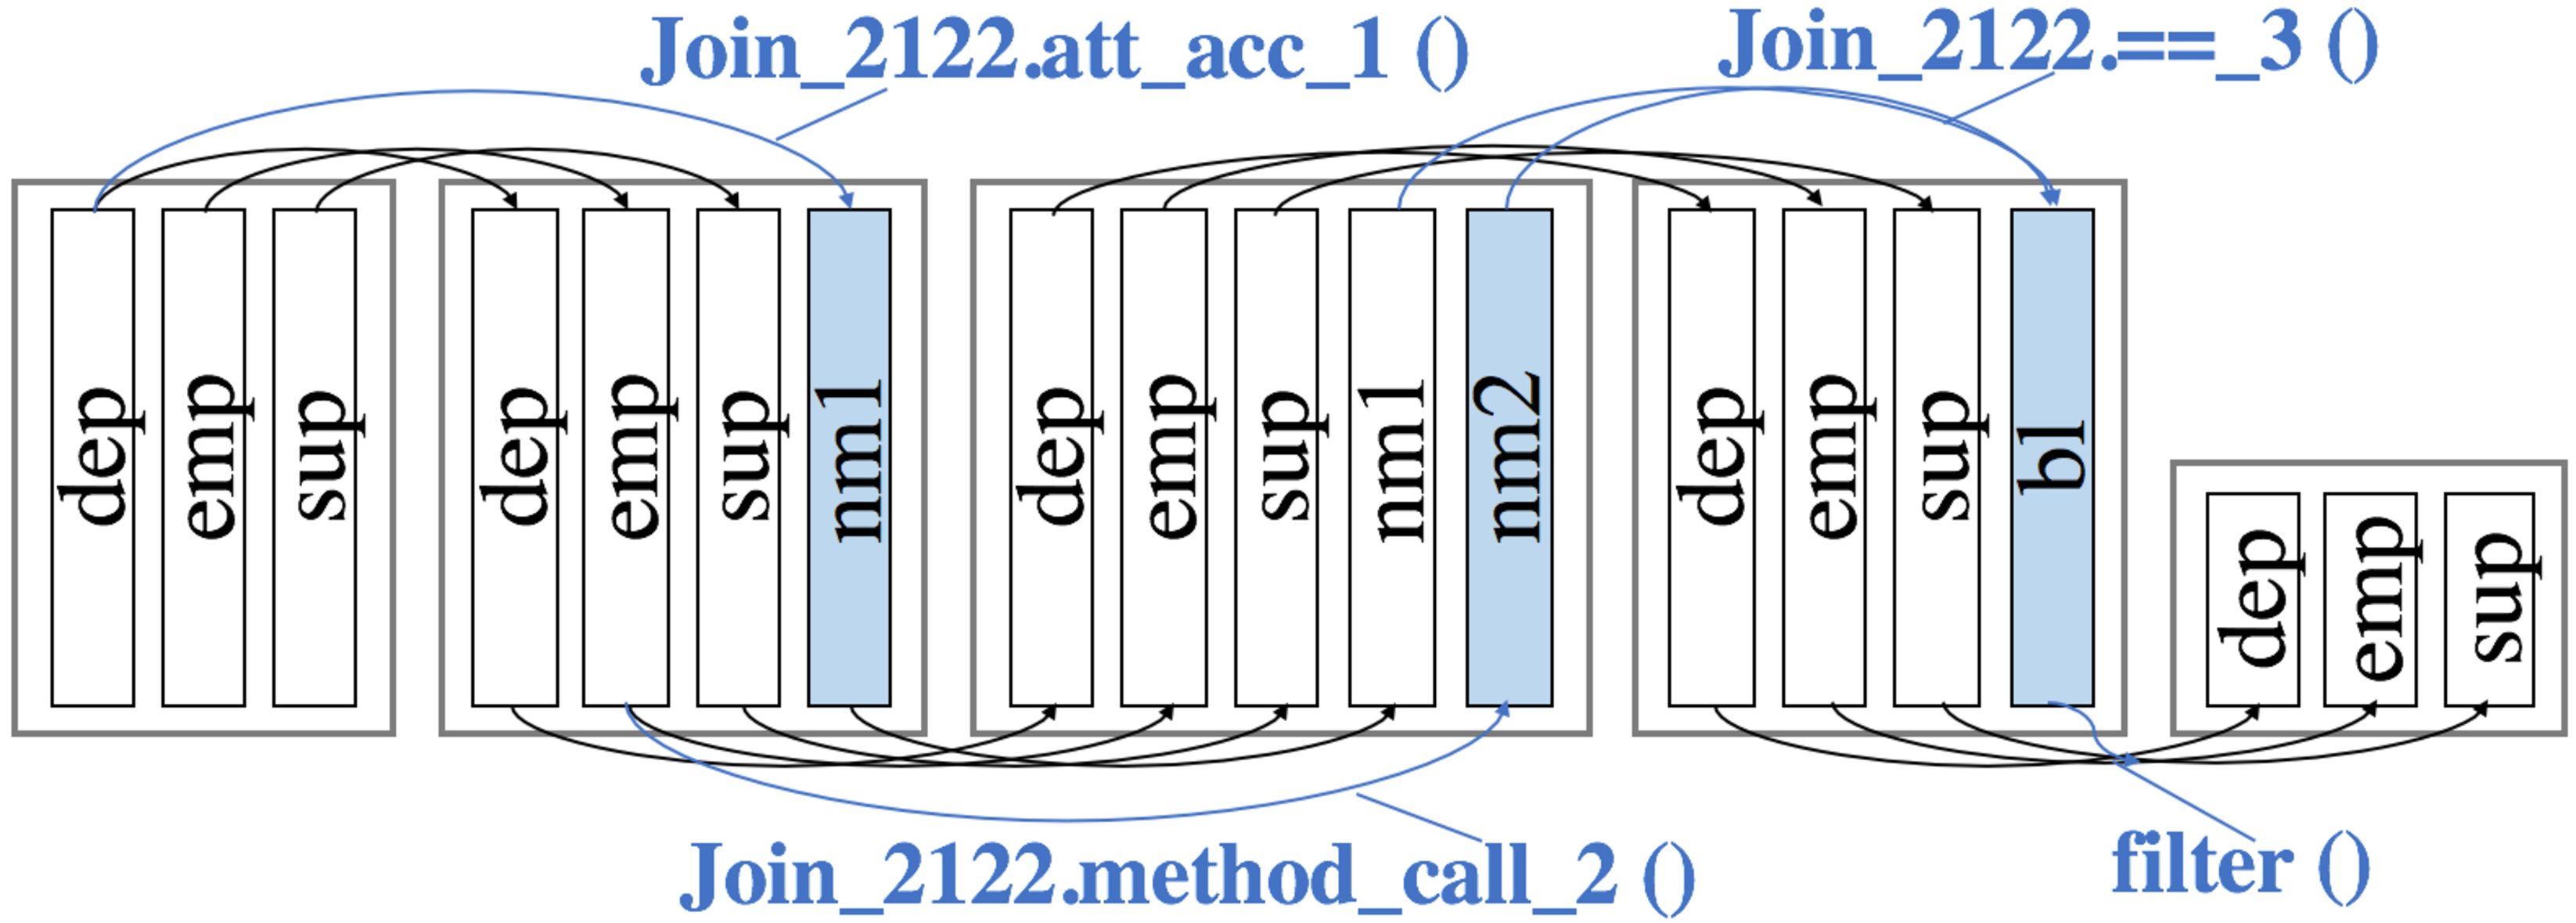
\includegraphics[width=3.3in]{TCAP}
  \end{center}
  \caption{Execution of the first four stages of a pipeline constructed from the example TCAP program.  The first two stages extract new vectors from 
existing vectors of objects, first via a call to
\texttt{Join\_2122.att\_acc\_1()}, which extracts
\texttt{Dep.deptName} from each item in the vector \texttt{dep}
of \texttt{Dep} objects, producing a new vector called \texttt{nm1}. Then,
via a call to \texttt{Join\_2122.method\_call\_2()}, which invokes \texttt{Dep :: getDeptName()} on each of the \texttt{Emp} objects
in the vector \texttt{emp}, producing a new vector called \texttt{nm2}.  A bit vector \texttt{bl} is formed by checking the equality of those two 
vectors via a call to \texttt{Join\_2122.==\_3()}, and then all of the vectors are filtered.}
  \label{fig:TCAP}
\end{figure}


\subsection{TCAP and Vectorized Execution} \label{sec:vectorized}

PC's vectorized execution engine repeatedly pushes 
so-called \emph{vector lists} through a series of pipeline stages.  Each pipeline stage
takes as input a vector list,
and produces a 
new vector list that consists of zero or more vectors from the input
vector list, as well as one or more vectors appended at the end of the list.
Pipeline stages are constructed in such a way that the overhead of a
virtual function call can be amortized on a vector list of objects,
aside from any virtual function calls that may be
present 
%(explicitly or perhaps implicitly in the form of memory management) 
in the user's code.
The TCAP language describes both the pipeline stages required to perform a PC computation, as well as the schema for each of the vector lists that
will be produced during the PC computation, and how each of the pipeline stages adds or removes vectors from the vector lists that are pushed through
the computation.

To see how this works through an example, consider a variant of the \texttt{getSelection()}:

\begin{codesmall} 
Lambda <bool> getSelection (Handle <Dep> arg1, 
     Handle <Emp> arg2, Handle <Sup> arg3) {
	return makeLambdaFromMember (arg1, deptName) == 
	       makeLambdaFromMethod (arg2, getDeptName); }
\end{codesmall}

\noindent PC compiles the lambda term resulting from a call to \texttt{getSelection()} into the following TCAP code:

\begin{codesmall}
WDNm_1(dep,emp,sup,nm1) <= APPLY(In(dep), 
   In(dep,emp,sup), 'Join_2212', 'att_acc_1', 
      [('type', 'attAccess'), ('attName', 'deptName')]);

WDNm_2(dep,emp,sup,nm1,nm2) <= APPLY(WDNm_1(emp), 
   WDNm_1(dep,emp,sup,nm1), 'Join_2212',
      'method_call_2', [('type', 'methodCall_2'), 
          ('methodName', 'getDeptName')]);

WBl_1(dep,emp,sup,bl) <= APPLY(WDNm_2(nm1,nm2),
   WDNm_2(dep,emp,sup), 'Join_2212', '==_3', 
      [('type', 'equalityCheck')]);

Flt_1(dep,emp,sup) <= FILTER(WBl_1(bl), 
   WBl_1(dep,emp,sup), 'Join_2212', []);
\end{codesmall}

\noindent
These four TCAP statements correspond to a pipeline of four stages,
as shown above in Figure \ref{fig:TCAP}.

This particular TCAP code begins with an \texttt{APPLY} operation, which is a five-tuple, consisting of: (1) the vector list and constituent
vector(s) for the \texttt{APPLY} to operate on, (2) the vector(s) from that vector list to copy
from the input to the output, (3) the name of the computation that the operation was compiled from, (4) the name of the compiled code (pipeline stage)
that the operation is to execute, plus (5) a key-value map that stores specific information about the operation that may be used 
later during optimization.

Specifically, in this case, the first \texttt{APPLY} in the TCAP computation describes a pipeline stage that
takes as input 
a vector list called \texttt{In}, which is made of the constituent vectors, referred to using 
the names \texttt{dep}, \texttt{emp}, and \texttt{sup}.
To produce the output vector list (called \texttt{WDNm\_1}), the vectors
\texttt{dep}, \texttt{emp}, and \texttt{sup} should be simply copied
(via a shallow copy similar with pointer assignment) from \texttt{In}.
In addition, the compiled code referred to by \texttt{Join\_2212.att\_acc\_1} will be executed via a vectorized application to the input
vector \texttt{dep}.  The result will then be put into a new vector called 
\texttt{WDNm\_1.nm1}.
The resulting vector list (consisting of the vectors shallow copied from the input as well as the new vector \texttt{WDNm\_1.nm1})
will be called \texttt{WDNm\_1}.  

Next, this TCAP program
specifies that \texttt{WDNm\_1} is processed by \texttt{APPLY}ing the
method call \texttt{getDeptName()} on the attribute \texttt{emp}; this is 
done via application of the compiled code referred to by \texttt{Join
  \_2212.method\_call\_2}.  
The vectors \texttt{dep}, \texttt{emp}, \texttt{sup}
and \texttt{nm1} are simply shallow-copied to the output vector list.

Then an equality check is performed to create \texttt{WBl\_1.bl}
(a vector of booleans) and the result is filtered based upon this
column.


Note that in each TCAP operation, the key-value map is only
informational and does not affect its execution.  However, this
information can be vital during optimization.  

\subsection{Template Metaprogramming}

In PC,
each vectorized pipeline stage (such as \texttt{Join\_2212.att\_ acc\_1}) is executed as fully-compiled native code, with no virtual function
calls.
In PC's C++ binding, this is accomplished by using the C++ language's extensive \emph{template metaprogramming} 
capabilities \cite{josuttis2012c++}.  Templates are the C++ language's way of providing generics functionality.
When a C++ template class or
function is instantiated with a type, %the instantiated template 
the C++ compiler actually generates optimized native code for that specific new type, at compile time.  
This is quite different from languages
such as Java, that must typically rely on slow virtual
function calls in order to implement generics.

To see how template metaprogramming is used by PC, consider
the TCAP operation from our example:

\begin{codesmall}
WBl_1(dep,emp,sup,bl) <= 
   APPLY(WDNm_2(nm1,nm2),WDNm_2(dep,emp,sup), 
      'Join_2212', '==_3', '');
\end{codesmall}

\noindent
Here, the pipeline stage \texttt{Join\_2212.==\_3} that is specified by the \texttt{APPLY} operation
actually refers to a function generated as a by-product of the
PC's \texttt{==} operation
in the line of code:

\begin{codesmall} 
return makeLambdaFromMember (arg1, deptName) == 
    makeLambdaFromMethod (arg2, getDeptName); 
\end{codesmall}

\noindent The \texttt{==} 
operation (corresponding to a higher-order function that
constructs a lambda term checking for equality in the output of two input lambda terms) is actually implemented as C++ template
whose two type parameters \texttt{LHSType} and \texttt{RHSType} are inferred from
the output types of the two input lambda terms. 
The \texttt{==} template returns an object of type \texttt{EqualsLambda} \texttt{<LHSType,} \texttt{RHSType>}, which
itself has an operation returning a pointer to the pipeline stage \texttt{Join\_2212.==\_3} referred to in the TCAP.
As expected, this stage processes in an input vector list,
creating a new vector of booleans, containing the truth values of the equality check of each \texttt{LHSType} from the left
input vector and each \texttt{RHSType} from the right input vector.
Using C++'s template metaprogramming facilities, this 
pipeline stage is generated specifically for \texttt{LHSType} and \texttt{RHSType} and optimized by the compiler for use with those
two types.  
As the \texttt{Join\_2212.==\_3} pipeline stage loops over the objects in the input vectors, 
there are no function calls that cannot themselves be inlined by the compiler
and optimized---unless, of course, the (potentially) user-defined equality operation over \texttt{LHSType} and \texttt{RHSType}
objects itself contains a virtual function call.

\eat{
\subsection{$k$-Means Example}

Now that we have described PlinyCompute at a high level, we turn to an example of what PlinyCompute looks like to a programmer.

Imagine that a user wished to use PC to build a high-performance library implementation of a $k$-means algorithm.
Once the programmer had defined the basic type over which the clustering is to be performed (such as the
\texttt{DataPoint} class), 
a programmer would likely next define a simple class that allows the averaging of vectors:

\begin{codesmall}
class Avg : public Object {
	long cnt = 1;
	Handle <Vector <double>> data = nullptr;
	Avg &operator + (Avg &addMe)
           {/* add addMe into this */}
};
\end{codesmall}

\noindent
The programmer might next add a method to the \texttt{DataPoint} class that converts the \texttt{DataPoint} object to an \texttt{Avg} object:

\begin{codesmall}
Avg DataPoint :: fromMe () {
	Avg returnVal;
	returnVal.data = data;
	return returnVal;
}
\end{codesmall}

\noindent
And also add a method to the \texttt{DataPoint} class that accepts a set of centroids, computes the Euclidean distance to
each, and returns the closest:

\begin{codesmall}
long DataPoint :: getClose (Vector <Vector <double>> 
        &centroids) {...}
\end{codesmall}

\noindent
Next, a programmer using PC would define an \texttt{AggregateComp} class using PC's lambda calculus, since, after all, the $k$-means algorithm is essentially 
an aggregation:

\begin{codesmall}
class GetNewCentroids : public AggregateComp 
    <Centroid, long, Avg, DataPoint> {

public:
   Vector <Vector <double>> centroids;

   Lambda <long> getKeyProjection (
       Handle <DataPoint> aggMe) override {
          return makeLambda (aggMe, 
              [&] (Handle <DataPoint> &aggMe) 
                 {return aggMe->
                     getClose (centroids);});
   }
   Lambda <Avg> getValueProjection (
       Handle <DataPoint> aggMe) override {
          return makeLambdaFromMethod 
              (aggMe, fromMe);
   }
};
\end{codesmall}

\noindent 
The declaration \texttt{AggregateComp <Centroid, long, Avg, DataPoint>} means that this computation aggregates
\texttt{DataPoint} objects.  For each data point, it will extract a key of type \texttt{long}, a value of type \texttt{Avg}, which will be
aggregated into objects of type \texttt{Centroid}.  To process each data point, the aggregation will use the lambdas constructed by
\texttt{getKeyProjection} and \texttt{get ValueProjection}.  
In this case, for example,
\texttt{getKeyProjec tion} builds a lambda which simply invokes the native C++ lambda given in the code---this
native C++ lambda returns the identity of the centroid closest to the data point.

To build a computation using this aggregation class, a programmer would need to specify the \texttt{Centroid} class (the result of this aggregation):

\begin{codesmall}
class Centroid : public Object {
	long centroidId; 
	Avg data;
public:
	long &getKey () {return centroidId;}
	Avg &getVal () {return data;}
};
\end{codesmall}

\noindent
And then build up a computation using these pieces:

\begin{codesmall}
Handle <Computation> myReader = 
    makeObject <ObjectReader <DataPoint>>
     ("myDB", "mySet");
Handle <Computation> myAgg = makeObject 
    <GetNewCentroids> ();
myAgg->centroids = ... // initialize the model
myAgg->setInput (myReader);
Handle <Computation> myWriter =  makeObject <Writer
     <Centroid>> ("myDB", "myOutSet");
    myWriter->setInput (myAgg);
pcContext.executeComputations (myWriter);
\end{codesmall}

\noindent After execution, the set of updated centroids would be stored in \texttt{myDB.mySet}.
Performing this computation in a loop, where the centroids are repeatedly updated until convergence, completes the implementation.


In our experience, for many applications such as Linear Algebra
Library, TPCH queries, or KMeans, PC codes require similar work in
terms of lines of source code to develop compared with equivalent codes using Spark's Scala binding, for
example, but require much lower effort to develop than using
object-oriented, C++ code without a declarative interface.

}

\section{Details of the PC Object Model} 
\label{sec:ObjectModel}

At the core of the system is the PC object model, which allows 
programmers to create, manipulate, and store persistent objects.
In keeping with our vision of granting programmers fine-grained control over how data are managed in the small, the PC object model
is much lower level than what is found in systems targeted more towards application programming, yet still provides a great deal of
key functionalities.

\subsection{PC Objects}

Arguably, the choice of how individual data items are to be represented and manipulated
in a data analytics or management system is one of the most
%consequential%
controversial decisions
that a system designer can make, both in terms of 
the programmability of the resulting system, and its performance.  For decades, the dominant model used in
data management was the flat relational model, which 
can achieve very good performance.
Flatness generally means 
that there is typically no distinction between the in-memory representation of data, and the on-disk (or in-network) representation of
data. Thus there is no (de-)serialization cost to move data to/from
disk and network, and memory management costs are very low. 

The downside is that flat relations are very limiting to a programmer.  Modern, object-based 
data analytics systems 
(such as Spark via its Resillient Distributed Dataset (RDD) interface \cite{zaharia2012resilient}) offer far more flexibility, at the (possible) cost of significant performance degradation.  
PC attempts to combine this flexibility with excellent performance.
The PC object model provides a fully object-oriented interface, supporting the standard functionality expected in a modern, object-oriented type system,
including generic programming (the PC object model supports generic Map and Vector types), pointers (or, more specifically,
``pointer-like'' objects called PC \texttt{Handle} objects), inheritance, and dynamic dispatch for runtime polymorphism.  

For example, imagine that the goal is implementing a distributed linear algebra system on top of the PC object model, where huge matrices are ``chunked'' into
smaller sub-matrices.  A sub-matrix may be stored via our current, C++ binding, using the following object:

\begin{code}
class SubMatrix : public Object {
public:
	int chunkRow, chunkColumn;
	int chunkWidth, chunkHeight;
	Vector <double> values; 
};
\end{code}

or, a sparse sub-matrix may be stored as:

\begin{code}
class SparseSubMatrix : public Object {
public:
	int chunkRow, chunkColumn;
	int chunkWidth, chunkHeight;
	Map <pair <int, int>, double> values; 
};
\end{code}

In the sparse sub-matrix, the \texttt{pair <int, int>} indexes a non-zero entry in the chunk by its row and column.

But while the PC object model provides a rich, object-oriented programming model, it also provides the good performance characteristic
of a flat relational model.
The key principle underlying the PC object model is \emph{zero-cost data movement}.  That is, once a data object
has been allocated and populated, moving the object to disk or across the network should be a simple matter of copying memory; there
should be no CPU cost for serialization and deserialization.

At first glance, it would seem to be impossible to offer zero-cost data movement while allowing a programmer to create and manipulate such objects.  
Pointers and container classes 
generally lead to high memory (de)allocation costs and high object (de)serialization costs, resulting in high CPU cost.
The PC object model avoids this 
by using a ``page-as-a-heap'' memory allocation model.  
The PC object model provides a call of the form:

\begin{code}
makeObjectAllocatorBlock (ptr, blockSize);
\end{code}

After such a call, \emph{all subsequent PC Object allocations by the thread creating the object allocation block will be performed directly to the memory
region starting at location} \texttt{ptr}.
Typically, when it runs a computation, PC's execution engine will obtain a page from its buffer pool to buffer output data, calling
PC's
\texttt{makeObjectAllocatorBlock ()} function with a pointer to the page where output data are to be written.  
When an action taken by the execution engine or user-supplied code causes an
out-of-memory execution, it means that the page is full.  At that point, the execution engine can take appropriate computation-specific 
action, such as creating 
an object allocation block out of a new (empty) page, writing the full page out to disk, sending it across the network, etc.  
No serialization or deserialization or any sort of post-processing of the page are needed, 
because all object allocations have taken place exclusively to the current allocation block.  

In order to guarantee zero-cost data movement,
one rule that a PC programmer must follow is that any object that will
be loaded into a distributed PC cluster must either be of a ``simple'' type (a simple type
must contain no raw C-style pointers and no 
virtual functions, and a \texttt{memmove}
must suffice to copy the object), or else it must descend from PC's \texttt{Object} class, which serves as the base for all complex object types.
Complex objects are those that include containers (\texttt{Vector}, \texttt{Map}) or pointer-like \texttt{Handle} objects.  Descending from PC's \texttt{Object} class
ensures that the resulting class type has a set of virtual functions
that allow it to be manipulated in and transferred across the
distributed PC cluster, 
such as a virtual deep copy function.  

\subsection{PC Handles}

To support linked data structures, dynamic allocation, and runtime polymorphism, it is necessary for a 
system to provide pointer-like functionality.  This is provided by PC's built-in \texttt{Handle} type.  
A \texttt{Handle} to an object is returned from a dynamic allocation to the current allocation block.
For example, a PC programmer 
can issue the statement:

\begin{code}
Handle <MatrixBlock> mySubMatrix = makeObject <MatrixBlock> ();
\end{code}

Internally, PC \texttt{Handle} objects contain two pieces of data: an \emph{offset pointer} that tells how far
the physical address of the object being pointed to is from the physical location of the 
\texttt{Handle}, and a \emph{type code} that stores the type of the
object that is pointed to.  

PC uses an offset pointer rather than a classical, C-style pointer in order to support
zero-cost data movement.  
A \texttt{Handle} may begin its life allocated
to one page, which may be stored on disk, then sent across a network
to another process.  
An actual C-style pointer
cannot survive translation from one process to another, as the program will be mapped to a different location in memory.
In contrast, at the new process, the \texttt{Handle} pointer
can function correctly. As long as the target of an offset pointer is stored in the same page, an offset pointer will be valid if the
page is copied in its entirety, including all \texttt{Handle}s and their targets.

\subsection{Dynamic Dispatch}
\label{sec:dyn_dis}

Supporting dynamic dispatch for virtual function calls is fundamental to the PC object model.
In PC, dynamic dispatch is facilitated by the type code stored within each
\texttt{Handle} object.
Each type code begins with a bit that denotes whether or not the referenced type is a simple type (which, by definition, cannot have any
virtual functions and for which a \texttt{memmove} suffices to perform a copy) or a type descended from PC's \texttt{Object} base class.
In the case of a simple type, the remaining bits encode the size of the referenced object.  

In the case of a PC \texttt{Object} or its descendants, the
type code is a unique identifier for the PC-\texttt{Object}-descended type of the object that the \texttt{Handle} points to.
In every major C++ compiler (GCC, clang, Intel, and Microsoft), virtual functions
are implemented using a virtual function table, or \texttt{vTable} object, a pointer to which is located at the beginning
of each C++ object having a virtual function.  Unfortunately, the \texttt{vTable} pointer is a native, C-style pointer, the
\texttt{vTable} pointer does not automatically translate when an
object is moved from process to process.  To handle this, in
PC's C++ binding, whenever a PC \texttt{Handle} object is dereferenced, 
a lookup on the
type code is performed transparently to the application programmer.  This lookup retrieves a process-specific pointer to that class' \texttt{vTable} object, which is
then placed at the head of the object.

Obtaining a pointer to a class' \texttt{vTable} object is not straightforward.
A user may run code on his/her machine that creates
a PC \texttt{Object}, and then ship that PC \texttt{Object} into the cloud.  At the other end, it arrives at a PC process that has never seen that type of object before and hence
does not have access to a \texttt{vTable} pointer for that class.
PC addresses this issue by requiring that all classes deriving from PC's \texttt{Object} base class be registered with the PC catalog
server before they are loaded into the distributed storage subsystem.  This registration requires shipping a library file (a \texttt{.so} file in Linux/Unix) to
the catalog server.  This library exposes a special
\texttt{getVTablePtr ()} function that returns a C-style raw pointer to the \texttt{vTable} for the class contained
in the \texttt{.so} file.

Whenever there is a \texttt{vTable} pointer lookup, the request first goes to the PC process' \texttt{vTable} lookup table.  When this 
lookup fails (because the process has not yet seen a \texttt{vTable} pointer for that class
type) the request then goes to the PC cluster's catalog server, which responds to the process with a copy of the appropriate \texttt{.so} file.  This 
\texttt{.so} file is then 
dynamically loaded into the process' address space, \texttt{getVTablePtr ()} is called, 
and the located \texttt{vTable} pointer is loaded into the lookup table, and then copied into the PC \texttt{Object} that is being referenced.  

In this way, PC provides something akin to the automated,
dynamic loading of classes (via Java Virtual Machine \texttt{.class} files) that is
provided by most big data systems.  
Objects of arbitrary type can be loaded into the distributed PC cluster and be processed using dynamically-loaded native code, as long
as the object type is registered first.

\subsection{Allocation, Deallocation, and Cross-Block Assignment}

There are three types of allocation blocks in PC, where an ``allocation block'' is a block of memory where PC \texttt{Object}s can be
allocated, or where they are located.

\begin{enumerate}

\item Each thread running in a PC process has exactly one \emph{active} allocation block, that is currently receiving allocations (all calls to
\texttt{makeObject} cause memory allocations to happen using that block).  Such an allocation block is created via a call to 
\texttt{makeObjectAllocatorBlock ()}.  User code typically creates and manipulates objects in this block.

\item Each thread also has one or more
\emph{inactive}, \emph{managed} blocks.  These are previously-active blocks of memory that contain one or more objects that are reachable
from some \texttt{Handle} that is currently in RAM.  When the number of reachable objects in an inactive, managed block drops to zero, it is automatically
deallocated.
When a user (or the PC system software) calls 
\texttt{makeObjectAllocatorBl ock ()}, the newly created allocation block becomes the active block, and if the previously-active allocation block has any
reachable objects on it, it becomes an inactive, managed block.

\item Finally, there are zero or more \emph{inactive},
  \emph{un-managed} blocks.  These are blocks with reachable PC
  \texttt{Object}s that are \emph{not} managed by the PC object model.  These tend to be pages of objects that have
been loaded into RAM from disk or across the network for processing
during a distributed computation.  Such blocks are paged in and out of the
buffer pool in much the same way as a relational database would page data in and out.
Rather than the PC object model being responsible for managing such blocks, PC's execution engine manages such blocks.
Further, since managed blocks are only managed by the ``home'' thread where
they are created, a managed block is effectively un-managed when viewed from
any other thread.

\end{enumerate}

In PC, each managed allocation block (active or inactive) has an active object counter (the number of objects that are reachable
from some \texttt{Handle} in RAM).  Each object in each managed allocation block (active or inactive) is reference counted, or pre-pended with a count of
the number of \texttt{Handle} objects that currently reference the object.  
Un-managed blocks (and objects inside of such blocks) are not reference-counted.

When the reference count on an object in a managed block goes to zero, it is automatically
deallocated (at least, this is the default behavior; it is possible for a programmer to override this behavior for speed, if desired, as we describe in Section~\ref{sec:allocation}).  
Once the number of reachable objects on an inactive, managed allocation block falls to zero, the block is automatically deallocated.  
In that sense, PC resembles a smart-pointer based memory management system.  

Since the fundamental goal of PC object model design is 
zero-cost data movement---an allocation block should be transferable across processes and immediately usable with no pre- or post-processing---one
potential problem is dangling \texttt{Handle}s.  Specifically: What happens when there is a \texttt{Handle} located in one allocation block that points to a PC
\texttt{Object} located in another allocation block?  The \texttt{Handle} may be valid, but when the \texttt{Handle}'s allocation block is moved to a new process where
the target block is not located, the \texttt{Handle} cannot be dereferenced without a runtime error. 
PC simply prevents this situation from ever happening. Whenever an assignment operation on \texttt{Handle} that is physically located
in the active allocation block results in that
\texttt{Handle} that is physically located in the active allocation block pointing outside of the block, a deep copy of the target of the assignment
is automatically performed.  This deep copy happens recursively, so any \texttt{Handle}s in the copied object that point outside of the active allocation block
have \emph{their} targets deep-copied to the active block.  For example, consider the following code:

\begin{code}
makeObjectAllocatorBlock (1024 * 1204);
Handle <Vector <double>> data = makeObject <Vector <double>> ();
for (int i = 0; i < 1000; i++)
     data->push_back (i * 1.0);
makeObjectAllocatorBlock (1024 * 1204); 
Handle <MatrixBlock> myMatrix = makeObject <MatrixBlock> ();
myMatrix->value = data; // deep copy of data happens!!
\end{code}

At the second \texttt{makeObjectAllocatorBlock}, the original allocation block, holding the list of \texttt{double}s pointed to by \texttt{data}, becomes
inactive.  The submatrix \texttt{myMatrix} is allocated to the new active block.  
Hence, the assignment of \texttt{data} to \texttt{myMatrix->value} is cross-allocation block, and a deep copy automatically happens to ensure that
the current block is zero-cost copy-able and movable.  

Such cross-block assignments require deep copies and are expensive,
but in practice, such they are rare, and a programmer who understands the cost can often avoid them, making sure to allocate
data that must be kept together to the same block.
Again, this is in-keeping with PC's design philosophy: trust the ability of the programmer to do the right thing, in the small.

\subsection{The PC Object Model and Multiple Threads}

While smart-pointer-based memory management
systems are often significantly faster than garbage collected systems, such systems still have their bottlenecks.  One of the bottlenecks is concurrency
control.
Since an object can have pointers across multiple threads, smart pointer counters must be locked before increment/decrement, which
can have a significant impact on performance.  PC, however, does not need to lock reference counts (or active object counts) because only managed blocks maintain
object reference counts and active object counts,
and a block can only be managed by a single thread.  
If a thread copies a \texttt{Handle} object referencing an object housed on another thread's managed block, 
the reference count will not be changed because from the copying thread's point-of-view, the allocation block is not managed.
This can, in theory, result in a problematic case where one thread has a \texttt{Handle} to an object that has been deallocated on the other thread (since
the reference count on the home thread will not be updated to reflect
the off-thread reference).  But in practice, it tends not to be a
problem.  Parallel and distributed processing is transparent to PC application
programmers, and they typically do not write explicitly multi-threaded code, so most cross-thread references happen as the result of computations staged by the 
PC execution engine.  The PC execution engine typically uses pages carefully so as to ensure that 
it is not possible for pages to be unpinned while references to them can still exist.

%\subsection{Data Loading}
%
%PC \texttt{Handle} objects also provide the basis for moving objects to the cloud.  A programmer first creates an allocation block, then
%creates a Vector to hold all of the objects, adds zero or more objects to the Vector, and sends the Vector to the cloud: 
%
%\begin{code}
%makeObjectAllocatorBlock (1024 * 1204);
%Handle <Vector <Handle <SparseSubMatrix>>> myVec = makeObject Vector <Handle <SparseSubMatrix>> ();
%Handle <SparseSubMatrix> storeMe = makeObject <SparseSubMatrix> ();
%myVec->push_back (storeMe);
%pcContext.createSet <SparseSubMatrix> ("Mydb", "Myset");
%pcContext.sendData <SparseSubMatrix> ("Mydb", "Myset", myVec);
%\end{code}
%
%All objects loaded to the cloud are loaded via \texttt{Handle} because then the objects can be manipulated in the cloud using
%runtime polymorphism.  It is fine when writing PC code to implicitly up-cast handles; a \texttt{Handle} object pointing to an object
%of any time can always be assigned to a \texttt{Handle <Object>} (or to a \texttt{Handle} to any type that is higher in the type
%hierarchy):
%
%\begin{code}
%Handle <SparseSubMatrix> storeMe = makeObject <SparseSubMatrix> ();
%Handle <Object> meTo = storeMe;
%\end{code}
%
%One of the basic polymorphic operations that must be over-ridden by all types descending from PC's \texttt{Object} class
%is \texttt{setupAndCopyFrom (void *, void *)} (in PC's C++ binding, this is done via macro expansion).
%This operation accepts as input a pointer to a target memory location large enough to store an object of the target type;
%the target memory location is first initialized (if needed), and then a deep copy from the source memory location is performed.
%PC uses this operation during data loading.  A PC process loading data views each set of newly-stored objects as a 
%\texttt{Handle <Vector <Handle <Object>>>}; it can then move those objects around via the assignment operator on 
%the \texttt{Handle} class, which in turn calls \texttt{setupAndCopyFrom} on the underlying type.


\section{Object Model Tuning}

\noindent
The PC object model is designed for zero-cost data movement, the result being that there is often no serialization or deserialization
cost
when moving PC \texttt{Object}'s across processes.  But memory management can still be costly.  Deallocating and cleaning
up complex objects (in particular, instances of container classes) can require significant CPU resources, which, depending upon the 
circumstance, may be un-necessary.  In-keeping with the assertion that application programmers should be in
control of performance-critical policies, it is possible to explicitly control how memory is reclaimed and re-used during PC computations.
This is facilitated through a set of \emph{allocation policies} that a programmer can choose from.

When the reference count for a PC \texttt{Object} located in a managed allocation block goes to zero, it is deallocated.  The exact
meaning of ``deallocated'' is controllable by the programmer, via a call to the \texttt{setAllocatorPolicy} on each computation object
that is created (\texttt{JoinComp}, \texttt{SelectionComp}, etc.).  Currently, PC ships with
three allocator policies:

\begin{enumerate}

\item Lightweight re-use.  This is the default policy.  When a PC \texttt{Object} is deallocated, its space in the allocation block is made available for re-use by
adding the space to a pool of similarly-sized, recycled memory chunks (all recycled chunks are organized into buckets, where a chunk of size
$n$ goes into bucket $\log_2 (n)$).  A request for RAM in a block is fulfilled by first scanning the recycled chunks in the appropriate bucket, then
attempting to allocate new space on the end of the block, if that fails.
\item No re-use.  The space containing deallocated PC \texttt{Object}s is not-reused.  Hence, it is very similar to classical, region-based allocation---though PC \texttt{Object}s
are reference-counted, and a destructor is called for each unreachable PC \texttt{Object}.
On the positive side, this allocation policy is very fast.  On the negative side, frequent allocations of temporary PC \texttt{Object}s will result in a lot of wasted space.
\item Recycling.  This is layered on top of lightweight re-use.  When the recycling allocator is used, any time a fixed-length
PC \texttt{Object} is deallocated, it is
added to a list of objects all having the same type.  All calls to \texttt{makeObject} with the zero-argument constructor will
pull an object off of the list of recyclable objects for the appropriate type.  
If an object is available for recycling, it is returned.  If not, or if any other constructor other than the zero-argument constructor is called, 
then the lightweight re-use allocator is used to allocate space for the requested
object.

\end{enumerate}

Note that
variable-length objects are never recycled.  There are just a few of these types in PC, and they are typically
used internally to implement the built-in PC container
types, and not by PC application programmers.  For example, PC's variable-length
\texttt{Array} class is used to implement the standard PC \texttt{Vector} container.  
These are not recycled because recycling allocations of such objects would need to match both on type and on size.  Matching on both at once would 
be computationally expensive, and could also allow long lists of objects to build up, waiting to be re-used.

In addition to policies that can be set on a per-computation basis,
it is also possible for a programmer to supply the following policies, on a per-\texttt{Object} bases, during PC \texttt{Object} allocation:

\begin{enumerate}

\item No reference counting.  This PC \texttt{Object} is not reference counted, and it is not included in the total count of objects on an allocation
block.  If each PC \texttt{Object} on an allocation block
is allocated in this way, this results in pure, region-based memory management, and is exceedingly lightweight.
\item Full reference counting.  This is the default.
\item Unique ownership.  The PC \texttt{Object} is not reference counted, but there can be one \texttt{Handle} object referencing the uniquely-owned
object.  When that \texttt{Handle} is destroyed, the object is deallocated.

\end{enumerate}




\section{Optimizing TCAP}
\label{sec:optimizer}

One of the key ideas driving the design and implementation of PlinyCompute is that \emph{all} PC computations should be optimized, both to
match programmer expectation---programmers generally expect
that changes in the way that boolean expressions are composed should not affect system runtime---and 
to protect against poor programmer choices when constructing the query graph.

Optimizability is one of the drivers for
the decision to compile all computations expressed in PC's lambda calculus into TCAP.  
TCAP resembles relational algebra, and it is similarly amenable to rule- and cost-based optimization
using a combination of methods from relational query optimization and classical compiler construction.
Currently, the optimizations implemented in PC are rule-based (such as pushing down selections).  We plan to work on cost-based optimization
in the future---this is a challenging research problem because of a lack of statistics over the data, which are arbitrary PC \texttt{Object}s.

PC's optimizer is currently implemented
in Prolog; a series of transformations are fired iteratively to improve the plan until the plan cannot be improved further.
For an example of the sort of optimization present in PC, consider the task of removing redundant method calls.  Imagine that a user
supplies a \texttt{SelectionComp} with the following \texttt{getSelection ()}:

\begin{codesmall} 
Lambda <bool> getSelection (Handle <Emp> emp) {
        return makeLambdaFromMethod (emp, getSalary) > 50000 &&
		makeLambdaFromMethod (emp, getSalary) < 10000;
}	
\end{codesmall}

\noindent PC would compile this into the following TCAP:

\begin{codesmall}
JK2_1(emp,mt1) <= APPLY(In(emp), In(emp), 'Sel_43', 'method_call_1',
  [('type', 'methodCall'), ('methodName', 'getSalary')]);

JK2_2(emp,bl1) <= APPLY(JK2_1(mt1), JK2_1(emp), 'Sel_43', '>_1', 
  [('type', 'const_comparison'), ('op', '>')]);

JK2_3(emp,bl1,mt2) <= APPLY(JK2_2(emp), JK2_2(emp,bl1), 'Sel_v3', 'method_call_2',
  [('type', 'methodCall'), ('methodName', 'getSalary')]);

JK2_4(emp,bl1,bl2) <= APPLY(JK2_3(mt2), JK2_3(emp,bl1), 'Sel_43', '<_1',
  [('type', 'const comparison'), ('op', '<')]);

JK2_5(emp,bl3) <= APPLY(JK2_4(bl1,bl2), JK2_4(emp), 'Sel_43', '&&_1', 
  [('type', 'bool_and')]);

JK2_6(emp) <= FILTER(JK2_5(bl3), JK2_5(emp), 'Sel_43', []);
\end{codesmall}

\noindent
This TCAP program first calls the method \texttt{getSalary ()} on \texttt{In::emp} to produce a new vector list \texttt{JK2\_2}, storing the result
of the method call in \texttt{JK2\_1.mt1}.  After comparing \texttt{JK2\_2.bl1} to \texttt{50000}, the result of the method call is dropped.
The method is then called once again on \texttt{JK2\_2.emp} and the result compared with \texttt{100000} to produce \texttt{JK2\_4}, at which 
point the two boolean vectors are ``anded'' and the result is filtered.

Obviously, there is a redundancy here as the method \texttt{getSalary ()} will be called twice.
If \texttt{getSalary} simply accesses a data member, the additional
call is costless.  But in the general case, a method call may run an arbitrary
computation.  Hence, the second call should automatically be removed as being redundant 
(by definition, all method calls evaluated during computation should
be purely functional, and so they must return the same value when called a second time).
The TCAP optimization rule leading to its removal is:

\begin{itemize}
\vspace{-5 pt}
\item If two \texttt{APPLY} operations are both of type \texttt{methodCall} and both invoke the same \texttt{methodName};
\vspace{-5 pt}
\item And one \texttt{APPLY} operation is the ancestor of the other in the TCAP graph;
\vspace{-5 pt}
\item And both \texttt{APPLY} operations operate over the same data object;
\vspace{-5 pt}
\item Then the second \texttt{APPLY} operation can be removed, and the result of the first \texttt{APPLY} carried through the graph.
\end{itemize}

\noindent
In our example, the
optimized
TCAP program is:

\begin{codesmall}
JK2_1(emp,mt1) <= APPLY(In(emp), In(emp), 'Sel_43', 'method_call_1',
   [('type', 'methodCall'), ('methodName', 'getSalary')]);

JK2_2(emp,mt1,bl1) <= APPLY(JK2_1(mt1), JK2_1(emp,mt1), 'Sel_43', '>_1', 
  [('type', 'const comparison'), ('op', '>')]);

JK2_4(emp,bl1,bl2) <= APPLY(JK2_3(mt1), JK2_3(emp,bl1), 'Sel_43', '<_1', 
  [('type', 'const comparison'), ('op', '<')]);

JK2_5(emp,bl3) <= APPLY(JK2_4(bl1,bl2), JK2_4(emp), 'Sel_43', '&&_1', 
  [('type', 'bool_and')]);

JK2_6(emp) <= FILTER(JK2_5(bl3), JK2_5(emp), 'Sel_43', []);
  
\end{codesmall}

\noindent
For another example of a rule-based TCAP optimization, 
consider the classical technique of pushing selection predicates past joins.  Imagine that a user supplied the following
\texttt{getSelection ()} for a \texttt{JoinComp} operation:

\begin{codesmall} 
Lambda <bool> getSelection (Handle <Emp> emp, Handle <Emp> sup) {
        return makeLambdaFromMethod (emp, getSalary) > 50000 &&
		(makeLambdaFromMethod (emp, getSupervisor) == 
                 makeLambdaFromMember (sup, name));
}	
\end{codesmall}

\noindent
Since all selection predicates are by default evaluated \emph{after} the join, 
this would be compiled to the following TCAP code:

\begin{codesmall}
JK2_1(sup,mt1) <= APPLY(InSup(sup), InSup(sup), 'Join_42', 'att_access_1', 
  [('type', 'attAccess'), ('attName', 'name')]);

JK2_2(sup,hash1) <= HASH(JK2_1(mt1), JK2_1(sup), 'Join_42', []);

JK2_3(emp,mt2) <= APPLY(InEmp(emp), InEmp(emp), 'Join_42', 'method_call_1', 
  [('type', 'methodCall'), ('methodName', 'getSupervisor')]);

JK2_4(emp,hash2) <= HASH(JK2_3(mt2), JK2_3(emp), 'Join_42', []);

JK2_5(sup,emp) <= JOIN(JK2_2(hash1), JK2_2(sup), 
  JK2_4(hash2), JK2_4(emp), 'Join_42', []);

JK2_6(sup,emp,mt3) <= APPLY(JK2_5(emp), JK2_5(sup,emp), 'Join_42', 'method_call_2',
  [('type', 'methodCall'), ('methodName', 'getSalary')]);

JK2_7(sup,emp,bool1) <= APPLY(JK2_6(mt2), JK2_7(sup,emp), 'Join_42', '>_1', 
  [('type', 'const comparison'), ('op', '>')]);

/* additional code here to check whether getSupervisor == name... 
   result goes into JK2_10.bool2 */

JK2_11(sup,emp,bool3) <= APPLY(JK2_10(bl1,bl2), JK2_10(sup,emp), 'Join_42', '&&_1', 
   [('type', 'bool_and')]);

JK2_12(sup,emp) <= FILTER(JK2_11(bool2), JK2_11(sup,emp), 'Join_42', []);
\end{codesmall}
 
\noindent
This code first uses \texttt{emp.getSupervisor ()} and \texttt{sup.name} to obtain the join keys. These are hashed, and 
a hash join is run (this is the \texttt{JOIN} operation).  After the hash join,
the result of calling \texttt{emp.getSuper visor ()} is compared with
\texttt{sup.name}.  If these two values are equal and the salary exceeds \texttt{50000}, the result tuple is accepted.

Clearly, it should be possible to first filter based off of the salary exceeding \texttt{50000} before the hash join is ever run.  Hence, one of
the rule-based optimizations available to PC is that:

\begin{itemize}

\vspace{-5 pt}
\item If there is a boolean predicate of the form $(b_1 \wedge b_2 \wedge ...)$ that operations
on the result of a join;

\vspace{-5 pt}
\item And some $b_i$ refers to values that depend only on one of the join inputs (in this case, \texttt{emp.getSupervisor ()}
\texttt{>} \texttt{50000};
depends only upon \texttt{emp});

\vspace{-5 pt}
\item Then $b_i$ can be pushed down to that join input, and a new
  \texttt{FILTER} is introduced.
\end{itemize}

\noindent In this case, after the transformation, we would have:

\begin{codesmall}
JK2_1(sup,mt1) <= APPLY(InSup(sup), InSup(sup), 'Join_42', 'att_access_1', 
  [('type', 'attAccess'), ('attName', 'name')]);

JK2_2(sup,hash1) <= HASH(JK2_1(mt1), JK2_1(sup), 'Join_42', []);

JK2_6(emp,mt3) <= APPLY(InEmp(emp), InEmp(emp), 'Join_42', 'method_call_2', 
  [('type', 'methodCall'), ('methodName', 'getSalary')]);

JK2_7(emp,bool1) <= APPLY(JK2_6(mt2), JK2_7(emp), 'Join_42', '>_1', 
  [('type', 'const comparison'), ('op', '>')]);

JK_2_7_1(emp) <= FILTER(JK2_7(bool1), JK2_7(emp), 'Join_42', []);

JK2_3(emp,mt2) <= APPLY(JK_2_7_1(emp), JK_2_7_1(emp), 'Join_42', 'method_call_1', 
  [('type', 'methodCall'), ('methodName', 'getSupervisor')]);

JK2_4(emp,hash2) <= HASH(JK2_3(mt2), JK2_3(emp), 'Join_42', []);

JK2_5(sup,emp) <= JOIN(JK2_2(hash1), JK2_2(sup), JK2_4(hash2), 
  JK2_4(emp), 'Join_42', []);

/* additional code here to check whether getSupervisor == name... 
   result goes into JK2_10.bool2 */

JK2_11(sup,emp,bool3) <= APPLY(JK2_10(bl1,bl2), JK2_10(sup,emp), 'Join_42', '&&_1', 
  [('type', 'bool_and')]);

JK2_12(sup,emp) <= FILTER(JK2_11(bool2), JK2_11(sup,emp), 'Join_42', []);
\end{codesmall}


\section{Experiments}

In this section, we describe our experimental evaluation of the
performance of the PC distributed computation system for a set of
representative big data analytics problems. The aim is to answer
following questions:

\begin {enumerate}
\item How useful is PC in building tools and libraries for big data analytics?
\item How efficient and easy is PC in manipulating highly nested and complex objects?
\item How well is PC in performing complex computations like real
  machine learning applications?
\end {enumerate}

\subsection {Experimental Environment and Applications}

All of the experiments reported in this paper were performed in a
cluster that consists of eleven Amazon EC2 m2.4xlarge machines,
running Ubuntu 16.04. Each machine had eight virtual cores, one SSD
disk, and 68 GB of RAM). One of the eleven machines served as the Master
node and the rest ten machines served as Worker nodes.

\vspace{5pt}
To conduct convincing benchmarks and performance comparisons, we
selected eight representative applications from three categories
of big data analytics workloads that are important for demonstrating
PC's utilities and performance:

\begin {itemize}
\item \texttt{Linear Algebra Library.} We constructed a linear algebra library
  and tested three common linear algebra computations: Gram Matrix,
  Linear Regression, and Nearest Neighbor Search.
\item \texttt{Analytical queries on TPC-H Data
    Set.}  We implemented two typical analytical queries against TPC-H
  benchmark data set that were denomalized to complex nested objects: the first one is an aggregation query reporting which customer buys which
  parts for each supplier; the second one is a Top-K similarity query
  to search for K customers who buy the closest items compared with a
  given customer.
\item \texttt{Machine Learning.} We also implemented three widely used
  iterative and complex machine learning algorithms: \textbf{Latent Dirichlet Allocation (LDA)}--A
  generative statistic model for text topic mining;
  \textbf{Gaussian Mixture Model (GMM)}--A clustering algorithm to generate a composite
  distribution whereby points are drawn from one of multiple Gaussian distributions;  and \textbf{KMeans}-- A well-known clustering algorithm that clusters
  data points into a pre-defined number of clusters.
\end {itemize}





\subsection {Construction of a distributed linear algebra library}
Since PC is designed to support the construction
of high-performance tools and libraries, our first benchmarking effort was aimed at determining 
whether PC is actually useful for that task.  Thus, we asked
a graduate student who knew nothing of PC to use the system to build a small Matlab-like 
programming language and library for distributed matrix operations.
We called this implementation \texttt{LilLinAlg}.

Our goal was to determine the 
performance and functionality that an expert programmer (but PC novice) could deliver in a short
timeframe, compared to a set of established distributed Big Data matrix implementations:
SciDB \cite{brown2010overview, stonebraker2011architecture} (built from the ground up by an MIT team over the last nine years), MLLib \cite{meng2016mllib} 
(the Big Data matrix
implementation shipped with Spark), and SystemML \cite{boehm2014hybrid, ghoting2011systemml, boehm2016systemml}
(a matrix and machine learning implementation developed
over the last seven years by a team at IBM, built on top of Spark and Hadoop).
The student spent about six weeks in this effort.

\subsubsection {Implementation}
In \texttt{LilLinAlg}, a distributed matrix is a PC dataset of dense matrix
blocks that is backed by one or more pages which can be buffered/cached in PC's distributed buffer pool and
persisted to PC's distributed user-level file system. Each dense matrix
block in the PC dataset is encapsulated as a MatrixBlock object that contains a
Vector of doubles and meta data that specifies the row and column
dimensions of this matrix block. All MatrixBlock in one distributed
matrix Set have equivalent row and column dimensions that can be
specified when a user claims a new distributed matrix dataset. A
MatrixBlock should be small enough to fit to a page (by default, page size
is 256 mega bytes).

\texttt{LilLinAlg} implemented common distributed matrix
computations on top of the PC platform, including $transpose$,
$inverse$, $add$, $substract$, $multiply$, $transposeMultiply$, $scaleMultiply$, $MinElement$,
$MaxElement$, $RowSum$, $ColumnSum$, $DuplicateRow$, $DuplicateCol$
and many more. Each computation can be translated to a partial PC query
graph. Taking $multiply$ for example, it will be translated to a partial
PC query graph that consists of a join and an aggregation like following:

\begin{code}
Handle <Computation> query1 = makeObject <LAMultiplyJoin> ();
query1->setInput (0, leftChild->evaluate(instance));
query1->setInput (1, rightChild->evaluate(instance));
Handle <Computation> query2 = makeObject <LAMultiplyAggregate> ();
query2->setInput(query1);
\end{code}

Here, the LAMultiplyJoin and LAMultiplyAggregate are both user-defined Computation classes that are
derived from the JoinComp class and AggregateComp class, which are
part of PC's declarative interface,  respectively. \texttt{LilLinAlg}
implemented the distributed matrix multiplication logic manipulating
two distributed matrixes (each is a dataset consists multiple
MatrixBlock objects that can be distributed across the cluster) through these
two user-defined classes. The LAMultiplyJoin
and LAMultiplyAggregate invoke numerical processing libraries such as
Eigen to manipulate MatrixBlock objects. Because each
MatrixBlock is backed by a Vector<double> Object, the pointer to the
raw array data is directly passed to Eigen library for efficient processing.

\texttt{LilLinAlg} also provided a linear algebra DSL for user to
easily express the linear algebra tasks in mathematical language. For
example, a least squares linear regression task can be easily coded as
\texttt{X = load(myMatrix.data); beta = (X '* X)\^{}-1 \%*\% (X '*
  y)}. 
In above DSL expression, \texttt{'*} represents a transposeMultiply computation,
\texttt{\^{}-1} represents an inverse computation, and \texttt{ \%*\%}
represents a multiply computation. 

\texttt{LilLinAlg} contained a compiler
to automatically translate the user program like above into a PC query graph that
connects (and optimizes) the partial PC query graphs corresponding to
each compuation to form the final query graph. Then it submits the
final query graph to the underlying PC platform for execution. 

In PC, the query
graph is automatically compiled to TCAP, which is then analyzed, optimized and compiled to native
code that gets executed in the PC distributed framework.

The \texttt{LilLinAlg} package consists of 3500+ lines of C++ code,
2700+ lines of C code that is automatically generated by yacc/lex, 
plus a few yacc/lex code.

\subsubsection {Experiments}

We ran three different computations:
a Gram matrix computation (given a matrix $\textbf{X}$, compute
$\textbf{X}^T \textbf{X}$), least squares linear regression (given a matrix of features $\textbf{X}$ and
responses $\textbf{y}$, compute 
$\hat{\pmb{\beta}} = (\textbf{X}^{T} \textbf{X})^{-1} \textbf{X}^{T} \textbf{y}$), and nearest
neighbor search in a Riemannian metric space \cite{lebanon2006metric} encoded by matrix $\textbf{A}$ (that is,
given a query vector
$\textbf{x}'$ and matrix $\textbf{X}$, find the $k$ rows in the matrix that minimize 
$d_{\textbf{A}}^2(\textbf{x}_i, \textbf{x}') = 
(\textbf{x}_i - \textbf{x}')^T\textbf{A}(\textbf{x}_i - \textbf{x}')$).  All experiments used
ten Amazon
EC2 m2.4xlarge workers.  

For Gram matrix and linear regression, SystemML V0.9 on Hadoop,
and Spark 1.6.1 was used; for
nearest neighbor, SystemML V1.0 on Spark and Spark 2.1.0 was used. We
use the same SciDB version 14.8 for all three
experiments.

For experiments on the PC platform, we mainly tuned the page size of the
distributed matrix dataset for different dimensions to make sure the
matrix can be fully distributed across the cluster:
we use 4 mega bytes page size for 10 dimensions, 16 mega bytes page
size for 100 dimensions, and 64 mega bytes for 1000 dimensions. In addition, PC's query optimizer dynamically decided to use
broadcast join when one input dataset of the join is smaller than two
giga bytes, and to use hash partition join when both input datasets of
the join is larger than two giga bytes.

For experiments on other platforms, we also carefully tuned the
systems for best performance. For example, we tuned Spark block size and repartition
size for every experiment. In SystemML, we also carefully chose to
use the parallel for loop, which boost performance significantly.

For
all three computations, 
$10^6$ data points were used. For each computation, 10, 100 and 1000
dimensions are tested.


\subsubsection {Results}

Results are given in 
Table \ref{fig:LR}. It shows for the most complex task, the nearest
neighbor computation, for both 100 and 1000 dimensions, PC
\texttt{LilLinAlg} provided the best performance compared with latest
SystemML, Spark and SciDB. It achieved $1.5\times$ speedup compared with
the next winner, the Spark-based
SystemML V1.0 with the latest version. For 10 dimension, PC performs slower
than SystemML, because SystemML runs small computation in local
mode. PC also achieved more than $10\times$ speedup compared with
Spark version 2.1.0, and $6\times$ speedup compared with SciDB version
14.8. 

For Gram Matrix and Linear Regression with high dimensions, PC achieved up to
$4\times$ speedup compared with the the Hadoop-based SystemML V0.9, up to $27\times$
speedup compared with Spark version 1.6.0, and up to $5\times$ speedup compared
with SciDB version 14.8.

We need point out that, although SystemML and Spark MLLib are
Java/Scala based, for their versions used
in all experiments, native
numerical librarires such as OpenBLAS are installed and invoked, so as to
the computation tasks, there is not much lanugage advantages that can
be taken by PC. Most performance benefits are from reduced
serialization/deserialization time with the PC object model, TCAP optimization and PC
backend's relational syle of processing objects.


\begin{table}[h!]
\begin{center}
\begin{tabular}{|c||c|c|c||c|c|c||c|c|c||}
\hline
& \multicolumn{3}{c||}{Gram Matrix} & \multicolumn{3}{c||}{Linear Regression} & \multicolumn{3}{c||}{Nearest Neighbor} \\
\hline
Dimensionality & $10$ & $100$ & $1000$& $10$ & $100$ & $1000$& $10$ & $100$ & $1000$ \\
\hline
\hline
PC (\texttt{LilLinAlg}) &00:07 & 00:09 &00:39 &00:14 &00:22 &00:49& 00:15 & 00:20 & 01:06 \\
SystemML &00:05$*$ &00:51 &02:34 &00:06$*$ &00:53 &02:38 &00:04$*$ &00:30 &01:32 \\
Spark \texttt{mllib} &00:20  &00:54 &17:31 &00:35 &01:01 &17:42 &01:20 & 04:49 &14:30 \\
SciDB   &00:03 &00:17 &03:20 &00:15 &00:33 &06:04 &00:28 &02:56 & 06:24 \\
\hline
\end{tabular}
\caption{Linear algebra benchmark. Format is MM:SS.
A star ($*$) indicates running in local mode.}
\label{fig:LR}
\end{center}
\end{table}

\subsubsection {Discussions}
This set of experiments demonstrated that a
domain-expert who has a few years' C++ programming experiences can fully control and
exploit the bare-metal computing power of PC through PC's highly
declarative and highly tunable interfaces.

In terms of performance, in every case except for the small problems when SystemML chose not to distribute the data,
\texttt{LilLinAlg} was the fastest.  
Though SystemML nearest neighbor approached the speed of 
\texttt{LilLinAlg}, we point out the vast difference in engineering effort between the two systems.  
SystemML was built over many years by a team of PhDs. Research papers have been written about the
technology developed for the system, including one awarded a VLDB best paper award \cite{boehm2016systemml}.
\texttt{LilLinAlg} was developed in six weeks, and it is faster (though to be fair, SystemML has a much broader
set of capabilities than \texttt{LilLinAlg}).

For productivity provided with the PC platform, we compared
\texttt{LilLinAlg} with Spark MLLib linalg
package~\cite{bosagh2016matrix}. Both packages offer similar linear algebra
functionalities. PC \texttt{LilLinAlg} has a DSL interface, is based on lower level
libraries like Eigen for numerical processing, and the developer 
wrote 3500+
lines of C++ code and 300+ lines of yacc/lex code. Spark linalg
package has no DSL and provides a lower level API-based interface. It
is based on JNI invocation to native BLAS implementations for
numerical processing. It consists of 3130 lines of scala
code. While it is true that scala is more compact and expressive
than C++, with PC's declarative interface, to develop a linear algebra
tool on top of PC requires similar coding efforts with using a
high-level language interface like Scala in Spark.



\subsection{Big object-oriented data manipulation}
For an example of the raw performance of the PC object model and its ability to power large-scale 
object-oriented computations, we use the TPC-H benchmark data set \cite{council2008tpc}
and de-normalize
the data into a large set of complex \texttt{Customer} objects. Each
\texttt{Customer} object contains, among
other data, a list
or \texttt{Order} objects, and each \texttt{Order} object contains a list of \texttt{Lineitem} objects,
each of which has a \texttt{Part} and \texttt{Supplier} object.  
We run two computations to manipulate such complex objects. First, we compute, for each supplier,
the set of parts that the supplier has sold to each customer (stored
as a map from customer name to a list of part identifiers).
Second, we compute the $k$ customers whose set of \texttt{Part} items purchased is closest to
a query set, according to Jaccard similarity.
The goal is to demonstrate the efficiency of the PC
Object model through comparison with equivalent implementations in Spark 2.1.0 platform.

\subsubsection{Implementation}
The \texttt{Customer}s per \texttt{Supplier} query consists of
following user-defined computations:  

\vspace{5pt}
1. \texttt{CustomerMultiSelection} is derived from the
declarative \texttt{MultiSelectionComp} interface to perform a flatmap
transformation and map each \texttt{Customer} object to one or more
\texttt{SupplierInfo} objects. Each \texttt{SupplierInfo} contains a
String member to specify the name of the supplier, a String member to
specify the name of the customer, an int member to specify a PartID, and
also a Map container that maps each customer name to a list of PartIDs
of \texttt{Part} items that are
ordered by this customer from this supplier. During the processing of
\texttt{CustomerMultiSelection}, the Map container is always empty and
it is mainly used for other computations.

The
\texttt{CustomerMultiSelection} customizes the flatmap logic as
following: for each \texttt{Customer} Object, it scans its list of
\texttt{Order} Object, and for each \texttt{Order} Object, it scans
its list of \texttt{LineItem} Object, then for each \texttt{LineItem}
Object, it creates a \texttt{SupplierInfo} Object using the customer
name of this \texttt{Customer} Object, supplier name of the
\texttt{Supplier} Object embeded in the \texttt{LineItem} Object, and
also the PartID of the \texttt{Part} Object that is also associated with
the \texttt{LineItem} Object. As mentioned, we leave the Map container
empty now.

\vspace{5pt}
2. \texttt{CustomerSupplierPartGroupBy} is derived from the declarative
\texttt{AggregateComp} interface to perform an aggregation on the
dataset of \texttt{SupplierInfo} objects. This customized computation
defines how to extract a Key (i.e. get the supplier name attribute
through method invocation) and a Value (i.e. a Handle to the \texttt{SupplierInfo} itself) from a
\texttt{SupplierInfo} object. 

The customerized computation also needs
to define how to aggregate the Values that share the same Key,  by
overloading operator+ of the Value type. For this query, we define the aggregation
logic for $lhsSupplierInfo + rhsSupplierInfo$ as following: if
$rhs$ has an empty Map container, it directly adds the
customerName to PartID mapping in the $rhs$ to the Map container in $lhs$, and
return $lhs$, which is to perform $V \rightarrow U$ aggregation;
and if $rhs$ has non-empty Map container, it iterates the Map
container in $rhs$ and adds each mapping to $lhs$'s MapContainer,
which is to perform $U \rightarrow U$ aggregation. In this fashion, we can
avoid create unnecessary Map container objects.

\vspace{5pt}
3. \texttt{CountAggregation} is the final aggregation to get the count of customers in the Map
container of each aggregated $SupplierInfo$ object. We add this
aggregation is mainly to be consistent with our Spark implementation
which requires an action in the end to trigger Spark to execute the
whole query graph.

\vspace{5pt}
The complete query graph is like following. 

\begin{code}
    Handle<Computation> myReader = 
        makeObject<ObjectReader<Customer>>("TPCH_db", "tpch_bench_set1");
    Handle<Computation> myFlatten = makeObject<CustomerMultiSelection>();
    myFlatten->setInput(myReader);
    {\bf myFlatten->setAllocatorPolicy(noReuseAllocator);}
    Handle<Computation> myGroupBy = makeObject<CustomerSupplierPartGroupBy>();
    myGroupBy->setInput(myFlatten);
    Handle<Computation> myWriteSet = 
        makeObject<CountAggregation>("TPCH_db", "t_output_set_1");
    myWriteSet->setInput(myGroupBy);
    pcContext.executeComputations (myWriter);
\end{code}

As highlighted in above code,  we find
that because the computation for \texttt{CustomerMultiSelection} needs
to allocate a lot of \texttt{SupplierInfo} Objects, reducing the CPU
overhead for memory allocation by setting the allocator policy to
noReuse can speed up the processing time by $2\times$.

\vspace{5pt}
The top-$k$ Jaccard stresses the PC Object Model in a similar way to
go through the list of \texttt{Order} Objects for each
\texttt{Customer} Objects, and then for each \texttt{Order} Object, go
through the list of \texttt{LineItem} Objects, and for
each\texttt{LineItem} Object, it gets the associated \texttt{Part}
Object to extract a PartID. 
The difference is that it implements a new user-defined computation
called \texttt{TopJaccard} to customize another declarative interface,
\texttt{TopKComp}. Compared with \texttt{CustomerMultiSelection}, it
requires less allocation of memory, because it transforms each
\texttt{Customer} Object into a CustomerID which is an Integer, and
also a Vector of Integers as the list PartIDs, which is much simpler
than a list of  \texttt{SupplierInfo} Objects. In addition, the
\texttt{TopJaccard} bounds the intermediate data size to top K
elements, which cause it generate less shuffle data compared with the
\texttt{CustomerSupplierPartGroupBy} computation.

\vspace{5pt}
The example of query graph for top-$k$ Jaccard query is as following:

\begin{code}
    Handle<Vector<int>> listOfPartIDs = 
          makeObject<Vector<int>>(199, 22, 34, 567, 1200, 37, 46, 459);
    Handle<Computation> myReader = 
         makeObject<ObjectReader<Customer>>("TPCH_db", "tpch_bench_set1");
    Handle<Computation> myTopK = makeObject<TopJaccard>(k, *listOfPartIDs);
    myTopK->setInput(myReader);
    Handle<Computation> myWriter = makeObject<Writer
          <TopKQueue<double, Handle<AllParts>>>>("TPCH_db", "result");
    myWriter->setInput(myTopK);
    pcContext.executeComputations (myWriter);
\end{code}

We also implemented equivalent TPC-H object model and queries in Spark. Because the data are object-oriented, it
is not possible to use Spark's Dataset/DataFrame abstraction to
implement this computation, so we mainly implemented TPC-H object model the two queries
using Spark RDD APIs in Java language.


\subsubsection{Experiments}
For this set of experiments, we mainly compare with algorithmically
equivalent  implementation on Spark version
2.1.0, using its high-level Java and RDD interfaces. As mentioned, we
find that the DataSet APIs in the same Spark version is insufficient
to support our required manipulation on the complex and nested
\texttt{Customer} objects.

On both platforms, we create a synthetic set of various number of \texttt{Customer}
Objects using a small TPC-H dataset created by DBGen using scale
factor 0.2. For both queries, we run the query against 2.4 million,
4.8 million, 9.6 million, 14.4 million, 19.2 million and 24 million
\texttt{Customer} Objects respectively. 

To measure the time on Spark for reading from in-RAM
deserialized RDD, we first apply a $distinct().count()$ operation to
the RDD of \texttt{Customer} Objects to make sure \texttt{Customer}
Objects are fully deserialized, before running each targeting query,
\texttt{Customer}s per \texttt{Supplier} or top-$k$ Jaccard. Then we
only report the latency for executing the targeting query.

Each experiment is run on the same 10-worker cluster as
afore-mentioned. On Spark platform, all data is
serielized using Kryo, parameters such as data partition size and parallelism are fully tuned to obtain
optimal performance. For Spark, 


\subsubsection{Results}


\begin{table}[h!]
\begin{center}
\begin{tabular}{|c||c|c|c|c|c|c|}
\hline
Kryo data size: &41.5GB & 83.1GB & 167.2GB &251.1GB &333.2 &416.2GB \\
\hline
& \multicolumn{6}{c|}{\texttt{Customer}s per \texttt{Supplier}} \\
\hline
PlinyCompute: hot Storage & 00:11&	00:19&	00:35&	00:51&	01:08&	01:21 \\
Spark: hot HDFS & 01:04&	01:53&	03:24&	04:54&	06:25&	08:16\\
Spark: in-RAM deserialized RDD & 00:16& 	00:29& 	00:56& 	01:21& 	02:18& 	03:56\\
\hline
& \multicolumn{6}{c|}{top-$k$ Jaccard} \\
\hline
PlinyCompute: hot Storage & 00:03&	00:03&	00:04&	00:05&	00:05&	00:06 \\
Spark: hot HDFS & 00:56&	01:38&	03:01 & 04:01&	05:22&	06:34\\
Spark: in-RAM deserialized RDD & 00:08& 	00:12& 	00:21 & 00:32& 	01:11& 	02:38\\
\hline
\end{tabular}
\caption{PlinyCompute vs. Spark for large-scale OO computation. Times in MM:SS.}
\label{fig:TPC}
\end{center}
\end{table}

Results are in Table \ref{fig:TPC},  and we see that when PC data are
stored in the PC's distributed Storage system and Spark data
are stored in
a hot HDFS, the computation is $6\times$ to $66\times$ faster in PC.  

If the data are already
fully deserialized and stored as an RDD, PC is 
between 50\% and $26\times$ faster.

From the results, we see that the processing time differences of the
two queries are more significant in PC compared with Spark. That's
mainly because for the \texttt{Customer}s per \texttt{Supplier} query,
it requires to allocate significantly more Objects than the top-$k$
Jaccard query: for each \texttt{Customer} Object, a
Vector$<$Handle$<$SupplierInfo$>$$>$ Object needs to be created in the
flatmap transformation, and to aggregate each \texttt{SupplierInfo}
Object, either a Map container needs to be created for a new Supplier,
or a Vector container needs to be created for a new Customer in each
Supplier, or a new PartID needs to be inserted into the Vector
container which may cause Vector to increase size by creating a new
larger Vector. Although we tune the allocation policy to alleviate
this allocation overhead, we can't reduce the deallocation
overhead. In top-$k$ Jaccard, less allocation/deallocation overhead
are involved.

As to Spark, because we tune the executor memory pool to be large
enough, the memory usage is low and JVM garbage collection activity is infrequent during query
processing. 
Therefore, compared with PC, Spark performance is less
sensitive to frequent creation of new Objects. 

This also indicate that PC may need new memory allocation policy to
avoid deallocation overhead when memory usage is low or to reduce
deallocation overhead by reusing objects.


\subsubsection{Discussions} 
The components of the TPC-H database are defined to
consist of eight separate and individual tables. After translated to
object-oriented data representation, a denormalized object is highly
nested and requires significant amount of dereference
operations to complete a query. Therefore, we regarded this set of
experiments as reasonable stress
tests for manipulating complex objects. 

The experimental results showed that
compared with Java objects, the PC
object model had a significant performance improvement, which were
brought by a couple of PC features such
as no serialization/deserialization overhead for moving data, and
relational syle of processing data in local storage, and can be
buffered across jobs.

In addition, as shown in Table \ref{fig:LOC}, the C++ implementations of two queries in
PC platform have slightly fewer lines of source code compared with
Spark Java implementations. While it is partially because we do not
need to write code for serializing and deserializing Objects (i.e. we did not
count kyro code, but we counted the user code for encoding and
registering a Kyro Object.), this also demonstrated that with a
declarative interface, implementing decision support
queries on complex and nested Objects can be easy even for using a low-level language like C++.

\subsection {Machine Learning}
\vspace{5pt}
\noindent
\textbf {(1) LDA.} We first describe our experience writing a word-based, non-collapsed LDA implementation \cite{jermaineExperimental} on top of
both Spark and PC.  LDA is a standard text mining algorithm and
non-collapsed. 
LDA is chosen because
it is challenging:
it contains two joins and two aggregations among other operations.
Our Spark combined RDD and DataSet        
implementation (using Spark 2.1.0) was carefully engineered by an expert.
On the cluster used before, we run LDA over a 2.5 million document
database.  Results (per iteration) are illustrated in Tab.~\ref{fig:LDA}:

\begin{table}[h!]
\begin{center}
\begin{tabular}{|c||c|c|c|c|c|c|}
\hline
PlinyCompute & \makecell{Spark 1: \\vanilla} & \makecell{Spark 2: also with \\join hint} & \makecell{Spark 3: also with \\forced persist} & \makecell{Spark 3: also hand-\\coded multinomial} \\
\hline
02:05 & 50:20 & 17:30 & 09:26 & 05:26 \\
\hline
\end{tabular}
\caption{PlinyCompute vs. Spark for LDA. Times in MM:SS, averaged over five iterations.}
\label{fig:LDA}
\end{center}
\end{table}
\vspace{-10pt}
While Spark performed well, the 
amount of work required to arrive at a good solution 
was significant, representing about a week of tuning.  First, among other things, our Spark expert had to force a 
broadcast join.  Then, it was necessary to force Spark to
persist the result of one of the joins for later use.  Finally, it was necessary to hand-code a 
Multinomial sampler to obtain an implementation that was competitive with PC.
This illustrates the advantage of PC's declarative approach: decisions such as broadcast vs. full hash
join as well as which intermediate results to materialize are
automated. 

\vspace{5pt}
\noindent
\textbf {(2) GMM.} A Gaussian mixture model (GMM) can be used to model data points that come
from one of $K$ clusters, and data points within the same cluster
can be modeled by a Gaussian distribution. So the $k$-th Gaussian
distribution is parameterized by a mean vector $\mu_k$ and a covariance
matrix $\sum_k$, and has a probability distribution $\pi_k$.

For this experiment, we
implemented GMM using the Expectation Maximization (EM) algorithm to be
consistent with the GMM algorithm implemented in Spark Mllib. EM is an
iterative optimization technique that consists of two steps in each
iteration: an estimation step to determine ``responsibility'' score
for assigning each data point to each Gaussian $k$ using the current model; and a maximization step to
update the model parameters using the new ``responsibility'' score. A complex
aggregation will run in each iteration to complete the two steps. The algorithm repeats
the two steps until log likelihood or parameters converges. 

We compared PC with Spark MLLib (using Spark 2.1.0) for $10^7$ data
points with 100 dimenisons, and $10^6$ data points with 300 and 500
dimensions. All experiments were run in the 10-worker cluster aforementioned. 
As illustrated in Tab.~\ref{fig:Gmm}, PC achieves a $2\times$ to
$3\times$ speedup compared with Spark MLLib. For Spark MLLib, we
carefully tuned the data partition size to make sure there are enough
partitions to keep all CPU cores busy.

\begin{table}[h!]
\begin{center}
\begin{tabular}{|c||c|c|c||}
\hline
Dimensionality & $100$ & $300$ & $500$ \\
Number of points & $10^7$ & $10^6$ & $10^6$ \\
\hline
\hline
PlinyCompute &00:33 & 00:53 & 2:16 \\
Spark \texttt{mllib} &1:41  &1:54 &5:05 \\
\hline
\end{tabular}
\caption{PlinyCompute vs. Spark for GMM. Times in MM:SS, averaged over five iterations.}
\label{fig:Gmm}
\end{center}
\end{table}
\vspace{-10pt}


\vspace{5pt}
\noindent
\textbf {(3) KMeans.} We developed a KMeans implementation on PC, which
is equivalent with the KMeans implementation in Spark MLLib. Spark
MLLib KMeans implementation has two initialization approach: KMeans++
and random initialization using sampling. For both experiments, we use
random initialization by sampling $K$ data points as initial
cluster centroids. For initialization, both implementations also compute $L^2$ norm for each data
point, and transform each data point into a new form with $L^2$ norm value
associated. 

Then in each iteration, each data point finds the closest cluster
of which the centroid has the closest distance with that data point, and assigns the closest
cluster label to itself. When computing the distance of a data point to a
centroid, a lower bound based on $\|a - b\| \geq |\|a\| - \|b\||$ is
first computed to avoid unnecessary distance computation. Then an aggregation is run to update centroids
based on computed new labels. Iteration repeats until centroids
converge.


We compared PC with Spark MLLib (using Spark 2.1.0) for $10^9$ data
points with 10 dimenisons, $10^8$ data points with 100 dimensions,  and $10^7$
data points with 1000
dimensions. All experiments were run in the 10-worker cluster aforementioned. 
As illustrated in Tab.~\ref{fig:KMeans}, PC achieved a $2\times$ to
$4\times$ speedup compared with Spark MLLib. 

\begin{table}[h!]
\begin{center}
\begin{tabular}{|c||c|c|c||c|c|c||}
\hline
& \multicolumn{3}{c||}{Initialization Latency} & \multicolumn{3}{c||}{Average
                                         Iteration Latency} \\
\hline
Dimensionality & $10$ & $100$ & $1000$ & $10$ & $100$ & $1000$\\
Number of points & $10^9$ & $10^8$ & $10^7$ & $10^9$ & $10^8$ & $10^7$\\
\hline
PlinyCompute &3:59 & 1:12 & 00:57 &00:37 & 00:09 & 00:06\\
Spark \texttt{mllib} &9:06  &4:18 &3:20 &01:02 & 00:28 & 00:23\\
\hline
\end{tabular}
\caption{PlinyCompute vs. Spark for KMeans. Times in MM:SS, averaged over five iterations.}
\label{fig:KMeans}
\end{center}
\end{table}


\vspace{5pt}
\noindent
\textbf{Summary.} For iterative and complex machine learning
benchmarks, compared with equivalent and carefully tuned implementations on the latest
Spark platform, PC still achieved $2 \times$ to $4 \times$
speedup. On one side this demonstrated PC's utility in handling
complex and iterative computations. On the other side, we've found that due to the complexity in mathematical and statistical
computations in those workloads, in many cases performance comparison is reduced to comparisons of
language efficiency and compiler supports. So it also indicates that PC has a
potential to achieve even larger performance gain by better
synergizing with C++ compiler and link-time optimizing tool chains.





\begin{table}[h!]
\begin{center}
\begin{tabular}{|c|c|c|}
\hline
Applications & LOC on PlinyCompute & LOC on Spark\\
\hline
Linear Algebra Package &3505& 3130 (scala)\\
TPC-H \texttt{Customer}s per \texttt{Supplier}&929 &953 (Java)\\
TPC-H top-$k$ Jaccard &793 & 966 (Java)\\
LDA &1038  &314 (Scala with Breeze)\\
GMM&932 & 474 (Scala with Breeze)\\
KMeans &695  &670 (Scala)\\
\hline
\end{tabular}
\caption{PlinyCompute vs. Spark: Lines of Source Code Comparison.}
\label{fig:LOC}
\end{center}
\end{table}




\section{Related Work}
\noindent
\textbf{Code Generation.} DryadLinq~\cite{yu2008dryadlinq} allows a user to express
distributed data flow
computations in a high-level language like C\# and strongly typed .NET
objects, and it compiles those computations into .NET assembler.
% Chris note: comparing with a relational system seems out of place
% Hyper~\cite{neumann2011efficiently} is a relational system,
% and it proposes a code
% generation strategy for query compilation to translate relational
% algebra to LLVM assembler for execution.  
LegoBase~\cite{klonatos2014building} switches the interface
from declarative SQL to a high-level language (Scala) and uses a query engine
written in Scala as a code generator to emit specialized and low-level
C code for execution. TupleWare~\cite{crotty2015tupleware} supports
multiple high-level languages (any language with an LLVM compiler) 
and aims to
optimize for UDFs by utilizing code
generation to integrate UDF code with the engine 
code. 
Weld~\cite{palkar2017weld} is a recent system developed in Scala and
Python. It proposes
a common runtime for data analytics libraries by asking library
developers to express their work using a new intermediate
representation (IR) and compiles this IR into multi-threaded code using
LLVM.  Then, application developers can use unified APIs to
call different libraries from Weld. Since version 2.0, Spark~\cite{zaharia2012resilient}
also exploits whole-stage code generation to generate JVM 
code.  The goal is mainly to reduce type parsing and virtual function call
overhead. PC uses a form of code generation (template metaprogramming) but 
the emphasis is quite different, in the sense that the goal is to allow for
efficient distributed programming with complex objects.

\vspace{5pt}
\noindent
\textbf{Optimized Memory Management.} 
Apache SparkSQL~\cite{armbrust2015spark} serializes 
relational table into byte arrays and stores the serialized bytes
in a main-memory columnar storage. Spark Tungsten~\cite{tungsten}
optimizes the Spark execution backend by grouping execution
data (such as hashed aggregation data) 
into byte arrays and data can be allocated off-heap via
the sun.misc.Unsafe API, reducing
GC overhead. Deca~\cite{lu2016lifetime} is a memory management framework aiming at
reducing GC overhead. It stores
various Spark data types, e.g. UDF variables, user data and
shuffle data into different
off-heap containers so that objects in each container can have a similar
lifetime and can be recycled together.
All of these methods attempt to alleviate GC overhead; in contrast, PC simply does
not use a managed runtime.

\vspace{5pt}
\noindent
\textbf{Relational Processing on Binary or Structured Objects.} 
Apache Flink~\cite{alexandrov2014stratosphere} uses reflection
to analyze Java/Scala object types, and it
maps each object type to one of a limited set of
fundamental data types to provide comparators to efficiently compare binary
representations and extract fixed-length binary key prefixes without
deserializing the whole object.

Spark~\cite{tungsten} has introduced the Dataset/Dataframe 
to encode JVM objects into relational binary data representation. 
Datasets/Dataframes enable relational-style processing
through a relational query optimizer called Catalyst and
also enables Java intermediate code generation to reduce virtual
function call overhead through Tungsten~\cite{tungsten}. 

Such techniques significantly boost performance, by moving away from a flexible, object-oriented
type of system to a more relational system.
It is known that relational systems can be fast, but they limit the sort of applications that
can easily be coded on top of the system.  In contrast, PC attempts to offer a fully 
object-oriented interface.

\vspace{5pt}
\noindent
\textbf{Native Systems.} 
Impala~\cite{bittorf2015impala} is a
C++-based 
SQL query engine that relies on Hadoop for scalability and 
flexibility in interface and schema. Impala compiles SQL 
into LLVM assembler.
However,
Impala uses a relational data model (though it can read/write
semi-structured data in storage formats such as Arvo, Parquet, RC and so
on from/to external storage such HDFS, using standard
serialization/deserialization methods).

Google Spanner~\cite{bacon2017spanner} is a distributed
database system with a SQL query processor. It implements a
dialect of SQL, which uses arrays and structures to
support nested data as a first class citizen. To integrate
with user applications, the relational data described needs to
be translated to protocol buffers or user languages. PC takes a fundamentally different approach, as all code is 
object-oriented rather an a mix of SQL and other high (or medium) level languages.

Tensorflow~\cite{abadi2016tensorflow} is a
distributed computing framework mainly designed for deep learning. It
mainly supports processing of numerical data with a
very limited set of types.
Tensorflow provides
a much lower level API than PC's declarative interface, based on tensors,
variables and sessions.




\section{Conclusions}

This paper has described PlinyCompute, or PC for short.  PC is a system for the development of high performance
distributed data processing tools and libraries.  PC is designed to inhabit the space between
high-performance computing platforms such as OpenMP and MPI, which provide little direct support
for managing very large data sets, and dataflow platforms such as Spark and Flink, which rely on 
a managed runtime to provide low-level services such as allocation and deallocation of data objects and memory management.
PC's guiding design principle is ``declarative in the large,
high performance in the small''.
In the large, PC presents the capable systems programmer with a very high-level, declarative interface, relying on automatic,
relational-database style optimization.  This is crucial for tool and library development, since the same tool should run well
regardless of the characteristics of the data and of the compute platform.  But in the small, PC relies on the PC object model.
The PC object model is an
API for storing and manipulating persistent data, and has been co-designed with PC's memory management
system and computational engine to provide maximum performance.
One of the key ideas behind the PC object model is the \emph{page as a heap principle}. All PC
Objects are allocated and manipulated in-place, on a system- (or user-) allocated page. There is no distinction
between the in-memory representation of data and the on-disk (or in-network) representation of data.
Thus there is no (de-)serialization cost to move data to/from disk and network, and memory management
costs are very low.

We have performed a reasonably extensive set of benchmark experiments that indicate that these ideas can result in 
a system that is very high performance and yet offers a relatively simple and usable object oriented API.  In particular, 
we have given strong evidence that PC \emph{is} particularly well-suited to tool and library development. 
For example, we asked a PhD
student (who at the outset knew nothing of PC) to use the system to build a small Matlab-like programming
language and library for distributed matrix operations called
\texttt{lilLinAlg}.  The resulting tool outperformed many other, long-lived tools
for the same purpose, such as SciDB, \texttt{mllib}, and SystemML.  SystemML in particular has resulted 
in several research papers,
including one awarded a VLDB best paper award \cite{boehm2016systemml}.
\texttt{lilLinAlg} was developed in six weeks by a single PhD student.
One may conjecture that had SystemML been built on a platform such as PC rather than on Spark, it might be significantly
faster than it is now.

Many avenues for future work remain.  In particular, there is significant scope for expanding the functionality and
usability of the PC object model, including relaxing the strict requirement that all \texttt{Handle}s point within a page.  This
would allow pointer-like objects to point off a page, perhaps even off of a machine.  

\bibliographystyle{ACM-Reference-Format}
\bibliography{pc} 

\end{document}
